\documentclass[iicol]{sn-jnl}
%%\documentclass[pdflatex,sn-nature]{sn-jnl}% Style for submissions to Nature Portfolio journals
%%\documentclass[pdflatex,sn-basic]{sn-jnl}% Basic Springer Nature Reference Style/Chemistry Reference Style
% \documentclass[pdflatex,sn-mathphys-num]{sn-jnl}% Math and Physical Sciences Numbered Reference Style
%%\documentclass[pdflatex,sn-mathphys-ay]{sn-jnl}% Math and Physical Sciences Author Year Reference Style
%%\documentclass[pdflatex,sn-aps]{sn-jnl}% American Physical Society (APS) Reference Style
%%\documentclass[pdflatex,sn-vancouver-num]{sn-jnl}% Vancouver Numbered Reference Style
%%\documentclass[pdflatex,sn-vancouver-ay]{sn-jnl}% Vancouver Author Year Reference Style
%%\documentclass[pdflatex,sn-apa]{sn-jnl}% APA Reference Style
%%\documentclass[pdflatex,sn-chicago]{sn-jnl}% Chicago-based Humanities Reference Style


\usepackage{graphicx}%
\usepackage{multirow}%
\usepackage{amsmath,amssymb,amsfonts}%
\usepackage{amsthm}%
\usepackage{mathrsfs}%
\usepackage[title]{appendix}%
\usepackage{xcolor}%
\usepackage{textcomp}%
\usepackage{siunitx}%
\usepackage{manyfoot}%
\usepackage{booktabs}%
\usepackage{algorithm}%
\usepackage{algorithmicx}%
\usepackage{algpseudocode}%
\usepackage{listings}%
\usepackage{adjustbox}%
\usepackage{tabularx}
\usepackage[numbers]{natbib}
\usepackage{multirow}     % Necessário para o \multirow
\usepackage{booktabs}  % For \toprule, \midrule, \bottomrule, \cmidrule

\raggedbottom
%%\unnumbered% uncomment this for unnumbered level heads

\begin{document}

\title[Article Title]{FOFF: An Energy-Efficient Task Offloading in VEC-Enabled Vehicular Networks Using Fuzzy
TOPSIS}

%%=============================================================%%
%% GivenName	-> \fnm{Joergen W.}
%% Particle	-> \spfx{van der} -> surname prefix
%% FamilyName	-> \sur{Ploeg}
%% Suffix	-> \sfx{IV}
%% \author*[1,2]{\fnm{Joergen W.} \spfx{van der} \sur{Ploeg} 
%%  \sfx{IV}}\email{iauthor@gmail.com}
%%=============================================================%%

\author*[1,2]{\fnm{Antônio Sérgio de Sousa} \sur{Vieira}}\email{sergio.vieira@ifce.edu.br}

\author[1,3]{\fnm{Alisson Barbosa de} \sur{Souza}}\email{alisson@ufc.br}
%\equalcont{These authors contributed equally to this work.}

\author[1]{\fnm{Joaquim} \sur{Celestino Júnior}}\email{joaquim.celestino@uece.br}
%\equalcont{These authors contributed equally to this work.}

\affil*[1]{\orgdiv{Intelligent Networks and Systems Group (INETSYS)}, \orgname{State University of Ceará}, \orgaddress{\street{Av. Dr. Silas Munguba, 1700}, \city{Fortaleza}, \postcode{60714-903}, \state{CE}, \country{Brazil}}}

\affil*[2]{\orgname{Federal Institute of Education, Science and Technology}, \orgaddress{\street{Av. da Universidade, 102}, \city{Itapipoca}, \postcode{62500-000}, \state{CE}, \country{Brazil}}}

\affil[3]{\orgname{Federal University of Ceará}, \orgaddress{\street{Av. José F. Queiroz, 5003}, \city{Quixadá}, \postcode{63902-580}, \state{CE}, \country{Brazil}}}

%%==================================%%
%% Sample for unstructured abstract %%
%%==================================%%

\abstract{
    In modern vehicular network environments, the demand for efficient data processing is crucial. However, this demand can exceed the computational capacity of the vehicles' On-Board Unit Interconnected (OBUI). One way to overcome these limitations is through edge devices with high computational capacity. Vehicular Edge Computing (VEC) facilitates the execution of these processing demands; however, latency remains a critical challenge. With advancements in 5G technology, research efforts have increasingly focused on determining whether tasks should be processed locally or offloaded to edge servers. Beyond latency considerations, energy consumption presents a significant concern for both OBUI and edge devices. This study introduces Fuzzy Offloading (FOFF), an innovative approach designed to balance these competing factors. Experiments show that FOFF reduces energy consumption and latency, achieving 72.11\% energy savings and 0.61\% lower processing time compared to the best greedy offloading approach considered. These results highlight FOFF’s efficiency in vehicular environments.
}
          
%%================================%%
%% Sample for structured abstract %%
%%================================%%

% \abstract{\textbf{Purpose:} The abstract serves both as a general introduction to the topic and as a brief, non-technical summary of the main results and their implications. The abstract must not include subheadings (unless expressly permitted in the journal's Instructions to Authors), equations or citations. As a guide the abstract should not exceed 200 words. Most journals do not set a hard limit however authors are advised to check the author instructions for the journal they are submitting to.
% 
% \textbf{Methods:} The abstract serves both as a general introduction to the topic and as a brief, non-technical summary of the main results and their implications. The abstract must not include subheadings (unless expressly permitted in the journal's Instructions to Authors), equations or citations. As a guide the abstract should not exceed 200 words. Most journals do not set a hard limit however authors are advised to check the author instructions for the journal they are submitting to.
% 
% \textbf{Results:} The abstract serves both as a general introduction to the topic and as a brief, non-technical summary of the main results and their implications. The abstract must not include subheadings (unless expressly permitted in the journal's Instructions to Authors), equations or citations. As a guide the abstract should not exceed 200 words. Most journals do not set a hard limit however authors are advised to check the author instructions for the journal they are submitting to.
% 
% \textbf{Conclusion:} The abstract serves both as a general introduction to the topic and as a brief, non-technical summary of the main results and their implications. The abstract must not include subheadings (unless expressly permitted in the journal's Instructions to Authors), equations or citations. As a guide the abstract should not exceed 200 words. Most journals do not set a hard limit however authors are advised to check the author instructions for the journal they are submitting to.}

\keywords{task offloading, energy optimization, fuzzy topsis, vehicular network}

%%\pacs[JEL Classification]{D8, H51}

%%\pacs[MSC Classification]{35A01, 65L10, 65L12, 65L20, 65L70}

\maketitle

\section{Introduction}\label{sec_introduction}
\newlength{\twocolumns}
\setlength{\twocolumns}{\dimexpr\columnwidth/2\relax} 

With the popularization and cost reduction of various communication technologies and high-capacity computational devices, interest in the development of vehicles capable of autonomous driving has also grown. However, creating technology for this purpose proves to be quite complex and challenging \cite{marko2021challenges}, specially within context of Intelligent Transportation Systems (ITS), where integrating autonomous vehicles with existing infrastructure and other vehicles demands innovative solutions to ensure efficiency, usefulness, reliability  and safety \cite{wang2023transportation}.

Building on this context, the development and evolution of 5G NR (Fifth-Generation Wireless Technology New Radio) and 6G (Sixth-Generation Wireless Technology) bring new application possibilities in the vehicular scenario. These solutions provide transmission speeds exceeding 20 Gbps and 1 Tbps \cite{morais20245g}\cite{tyagi20256g}, respectively. Additionally, transmission latency, which in 5G NR is approximately 1 ms \cite{morais20245g}, will be reduced to the microsecond range in 6G (approximately 5~$\mu$s) \cite{tyagi20256g}, driving the adoption of autonomous vehicles (AVs) in our daily lives. Thus, these technologies foster the development of real-time applications essential for the safe and efficient operation of autonomous vehicles in complex environments. However, as latency decreases, a new challenge emerges: the need to process the massive influx of data quickly and efficiently.

As high communication latency becomes less of an issue for real-time applications, it is important to consider solutions capable of processing large volumes of data with minimal response times while simultaneously reducing energy costs \cite{katare2023survey}. In this context, several proposals have been presented, particularly those emphasizing the use of more robust processing devices than those installed in vehicles. Among these proposals, Vehicular Edge Computing (VEC) stands out, as it integrates Mobile Edge Computing (MEC) into vehicular networks by moving computation, communication, and storage resources closer to vehicles, thus enabling lower latency and reduced bandwidth consumption \cite{liu2021vehicular}.

However, despite these approaches related to infrastructure, determining when and where to offload large volumes of data is crucial for meeting the computational demands of applications in autonomous vehicular environments. Additionally, it is equally important to achieve a balanced distribution of the overall system workload. This decision-making process is known as \textit{task offloading} \cite{kumari2022task}.

The task offloading strategies typically fall into two categories: binary offloading and partial offloading. The binary offloading determines whether a task should be processed locally or completely offloaded \cite{duan2024binary}, \cite{guo2023intelligent}. In contrast, the partial offloading allows tasks to be divided and assigned to edge and local computing simultaneously \cite{kuang2019partial}, \cite{ren2017partial}.

Several studies in this field have been proposed to minimize processing time and energy consumption in vehicular environments. Optimization problems of this nature have been addressed by various strategies, such as greedy algorithms \cite{de2022context}, metaheuristics \cite{abuthahir2024tasks}, and reinforcement learning \cite{fofana2024intelligent}. Nevertheless, we consider that employing fuzzy logic, a method designed to handle imprecise environments, could lead to  a novel approach in highly dynamic scenarios. Unlike classical logic, fuzzy logic offers a gradual representation of truth, which is particularly advantageous for decision-making processes based on uncertain or imprecise information \cite{zadeh1965fuzzy}.

The proposal of this work is to create an efficient solution to determine the best processing alternative, considering the balance between task offloading latency and energy consumption at the processing devices. This involves deciding whether it is more advantageous to process the data locally or to offload it, taking into account factors such as data upload time, server queue wait time, processing time, and the time required to retrieve processed data.

To achieve this, we utilize a fuzzy logic-based technique called Fuzzy TOPSIS (Fuzzy Technique for Order Preference by Similarity to Ideal Solution) \cite{CHEN20001}, which is capable of generating a ranking of the best options for multi-criteria decision-making problems. Our approach aims to quickly balance conflicting objectives to provide better decision support in challenging vehicular scenarios.

The Fuzzy TOPSIS method was selected due to its stability and lower computational complexity \cite{adali_alternative_2016} compared to alternative fuzzy ranking techniques, such as Fuzzy AHP (Fuzzy Analytic Hierarchy Process) \cite{chang_applications_1996} and Fuzzy PROMETHEE (Fuzzy Preference Ranking Organization Method for Enrichment Evaluations) \cite{adali_alternative_2016}. This stability in response to the addition or removal of alternatives is crucial in dynamic vehicular systems. As demonstrated by Lima Junior et al. \cite{lima_junior_comparison_2014}, introducing a new alternative significantly altered the rankings produced by Fuzzy AHP, whereas Fuzzy TOPSIS maintained consistent results under identical conditions. Furthermore, Fuzzy AHP incurs substantial computational overhead due to its requirement for multiple pairwise comparisons and weight recalibrations whenever the set of alternatives changes. 

While Fuzzy PROMETHEE can be effective in static or subjective analysis scenarios, it suffers two critical drawbacks for real-time decision-making: first, it depends on predefined preference functions, i.e., parameters that must be manually tuned for each criterion and cannot autonomously adapt to rapid fluctuations in latency, processing load, or vehicle mobility; second, its often yield partial rankings by grouping indistinguishable alternatives into equivalence levels, forcing the use of additional tie-breaking procedures and adding both latency and complexity. These limitations weaken its flexibility, increase configuration overhead, and compromise both the speed and scalability required in highly dynamic VEC environments. In contrast, Fuzzy TOPSIS provides a complete ranking with computational complexity linear in the number of alternatives, enabling rapid and stable decision-making.

To analyze the effectiveness of our proposal, we developed a vehicular scenario consisting of a vehicle capable of communicating with five edge devices through 5G (Fifth-Generation Wireless Technology) communication. Each device, including the OBUI, has a different computational capacity. We intentionally included two edge servers with high computational capacity but significant energy consumption to evaluate whether the solutions proposed in other studies effectively address this type of problem. In summary, our main contributions are:

\begin{enumerate}
    \item Development of an innovative task offloading solution based on Fuzzy TOPSIS to balance energy consumption and task completion time.
    \item By integrating latency, energy consumption, and computational resource availability into its decision-making process, our solution effectively addresses conflicting objectives in dynamic vehicular scenarios.
   \item Demonstration of FOFF's adaptability across different scenarios (challenging and balanced) without requiring manual parameter tuning.
   \item Unlike metaheuristic and reinforcement learning approaches, our solution does not require a training phase or iterations to converge to a satisfactory solution.
\end{enumerate}

In Section \ref{sec_related_work},  and \ref{sec_system_model}, we describe respectively the related works, and the key aspects considered in modeling the simulated environment. Section \ref{sec_fuzzy_topsis} details our proposed solution. In Section \ref{sec_experiments}, we present the experiments, sensitivity analysis and results, and finally, the conclusion is provided in Section \ref{sec_conclusion}. Moreover, the definitions of the acronyms are presented in Table \ref{tab:acronyms}.

\begin{table*}[h!]
    \scriptsize
    \centering
    \caption{Acronyms – List of the acronyms and abbreviations used throughout the article.}
    {\setlength{\tabcolsep}{2pt} % Reduz o espaço entre siglas e descrições (colunas 1-2 e 3-4)
    \renewcommand{\arraystretch}{1.2}    
    \begin{tabularx}{\textwidth}{p{0.09\textwidth}@{\hskip 2pt}>{\raggedright\arraybackslash}p{0.42\textwidth} p{0.09\textwidth}@{\hskip 2pt}>{\raggedright\arraybackslash}p{0.39\textwidth}}
    \toprule    
    5G & Fifth-Generation Wireless Technology & MABS & Macro Base Stations\\      
    A3C & Asynchronous Advantage Actor-Critic & MCDM & Multi-Criteria Decision-Making\\
    AHP & Analytic Hierarchy Process & MEC & Mobile Edge Computing\\
    C-V2E & Cellular-Vehicle to Everything & MIBS & Micro Base Stations\\
    DDPG & Deep Deterministic Policy Gradient & NIS & Negative Ideal Solution\\
    DQN & Deep Q-Network & OBUI & On-Board Unit Interconnected\\
    DRL & Deep Reinforcement Learning & PER & Priority Experience Replay\\
    DSRC & Dedicated Short Range Communication & PIS & Positive Ideal Solution\\
    FFDU & First-Fit Decreasing Utilization & \\
    FOFF & Fuzzy Offloading & PROMETHEE & \\
    && & Preference Ranking Organization Method\\
    && & for Enrichment Evaluations\\
    FP-Sched & Fully Partitioned Scheduling & ROFF & Random Offloading\\
    GTT & Greedy Task by Task & SNR & Signal-to-Noise Ratio\\
    TFN & Triangular Fuzzy Number & TOPSIS & Technique for Order Preference by Similarity to Ideal Solution\\
    VEC & Vehicular Edge Computing & WAVE & Wireless Access in Vehicular Environments \\
    \bottomrule
    \end{tabularx}
    }
    \label{tab:acronyms}
\end{table*}


\section{Related Work}\label{sec_related_work}
The importance of research in vehicular environments is widely recognized, as observed through various studies, such as \cite{bi2023back}, \cite{zhang2022vehicular}, \cite{guo2024deep}, \cite{mirza2023drl}, and \cite{alam2024energy}. Addressing challenges in highly dynamic environments is a critical aspect for enabling the deployment of autonomous vehicles.

There will always be applications that increasingly consume computational resources as new demands arise. In this context, the importance of techniques aimed at optimizing the use of computational and energy resources to make these applications viable becomes evident.

With this in mind, in this section, we present some studies that employ new techniques to try to overcome these challenges in vehicular environments. However, these techniques fail to address a critical aspect: situations where the energy costs is significantly higher than the cost related to computational latency. This imbalance can lead to various sustainability issues affecting the viability of vehicular environment infrastructure, substantially increasing operational costs.

In the study conducted by \cite{sarieddine2022opportunistic}, a framework is proposed for a clustered vehicular environment, capable of delegating the offloading decision to the clusterhead, thus improving scalability and reducing network traffic. The core of the proposal is based on a decision-making strategy that considers SNR (Signal-to-Noise Ratio) and the time required to send an offloading request. However, the study does not thoroughly explore clustering techniques or consider the energy consumption of edge devices.

In \cite{ko2023belief}, an approach was used to create a probability distribution based on a partially observable Markov Decision Process to estimate information about the conditions of communication channels and the computational resources available on edge servers. The proposed algorithm (BTOA - Belief-based Task Offloading Algorithm) successfully reduced the total latency for task completion by 42\% compared to other tested algorithms. However, energy consumption and load balancing was not considered.

Some studies primarily focus on meeting latency constraints to satisfy application requirements. For this purpose, it was also observed that some solutions include proposals to improve the utilized network architecture. This is the case in the work presented in \cite{lu2023a3c}. The study developed a vehicular edge computing architecture based on SDN (Software-Defined Networking), aiming to enable more effective computational resource management. In addition to the SDN architecture, the authors designed a task offloading decision algorithm, aware of load balancing, based on A3C (Asynchronous Advantage Actor-Critic) \cite{mnih2016asynchronous} and Deep Reinforcement Learning. Simulations demonstrated that the proposed approach effectively distributed workloads among edge servers, reduced latency, and improved the task completion ratio. Once again, energy consumption was not considered.

In the study conducted in \cite{guo2024deep}, two techniques were integrated to seek an optimal task offloading policy. Deep Deterministic Policy Gradient (DDPG) was combined with Priority Experience Replay (PER) to achieve this goal. According to the authors, the approach converged more quickly than other algorithms tested in real-time environments. However, the technique developed requires improvements related to adaptability and scalability.

In \cite{wu2024efficient}, a many-objective solution called MaOITGO-CO is proposed for managing task offloading in diverse vehicular edge networks. This solution uses principles from invasive tumor growth to optimize task completion time, energy consumption, resource costs, and load balancing. According to the authors, simulation results indicate that MaOITGO-CO outperforms other solutions in terms of convergence and diversity. The simulations results reveal that the algorithm achieves significant reductions in energy usage by optimizing task offloading decisions. However, the algorithm's complexity may pose challenges in rapidly changing vehicular scenarios.

The authors in \cite{sharma2024intelligent} proposed a solution based on Deep Reinforcement Learning, utilizing both off-policy (DQN - Deep Q-Network) and on-policy (A3C - Asynchronous Advantage Actor-Critic) approaches. The DQN method was employed to enable effective learning for task offloading through historical data while A3C was adapted to explore new policies. The objective is to provide a solution that attains an equilibrium between exploration and stability. Through experiments, the authors demonstrated the improvements in the average reward during iterative training. However, the complexity of the model and the need for continuous training may limit its applicability in highly dynamic environments.

In the study conducted by \cite{sharma2024edge}, the authors proposed a two-stage solution for edge server selection in the context of task offloading from mobile devices in industrial IoT networks. In the first stage, the matching feasibility between mobile devices and edge servers is verified using Hall's Marriage Theorem. This step involves constructing a bipartite graph where each mobile device is associated with a list of preferred edge servers. In the second stage, once the matching feasibility is confirmed, a server selection algorithm is employed to assign tasks optimally. This algorithm considers both the computational capacity and the proximity of the edge servers, prioritizing mobile devices based on task-specific parameters such as processing requirements and execution deadlines. Simulation results demonstrate that this dual-stage approach minimizes energy consumption and overall time delay. However, in the first stage, the ranking of preferred servers does not account for high energy consumption, potentially selecting servers with high computational capacity but excessive energy usage.

In summary, the key aspects of the related works are presented in Table \ref{tab:comparison_offloading}.

\newlength{\coluna}
\setlength{\coluna}{\dimexpr\textwidth/5\relax} 

\begin{table*}[!ht]
    \renewcommand{\arraystretch}{1.3}
    \setlength{\tabcolsep}{2.5pt}    
    \scriptsize
    \centering
    \caption{Comparison of Offloading Solutions – A comparative assessment of the offloading strategies proposed in previous studies.
    }
    \begin{tabular}{cp{\coluna}p{\coluna}p{\coluna}p{\coluna}}
        \toprule
        \bfseries Ref. & \bfseries Strategy & \bfseries Communication Technology & \bfseries Achievement & \bfseries Limitation \\
        \midrule
        \cite{sarieddine2022opportunistic} & Opportunistic task assignment using vehicular fog environment. Clustering and offloading decision based on SNR & DSRC and ZigBee & Low latency by utilizing mobile computing nodes & Limited scalability for high-density traffic scenarios. It does not take into account energy consumption or explore other clustering techniques \\ 
        \cite{lu2023a3c} & A3C-based DRL & C-V2E and DSRC & Improved load balance, delay performance, and task completion ratio & Energy efficiency optimization not fully addressed \\ 
        \cite{ko2023belief} & Belief-based offloading using POMDP (Partially Observable Markov Decision Process) & NA & Reduced total latency by 42\% compared to conventional algorithms & Energy consumption not considered \\ 
        \cite{xu2022computation} & Deep Deterministic Policy Gradient (DDPG) and Priority Experience Replay (PER) & 5G & Accurate traffic flow prediction; reduced energy and delay & High computational overhead for model training \\ 
        \cite{wu2024efficient} & Invasive Tumor Growth Optimization (ITGO) & MIBS and MABS & Optimized delay, energy, and load balance with Pareto solutions & Complexity in managing many objectives in real-time scenarios \\ 
        \cite{sharma2024intelligent} & DRL (DQN and A3C) & NA & Improved average reward during iterative training & Continuous training required for model adaptation \\
        \cite{sharma2024edge} & Two-stage edge server selection & NA & Minimized energy consumption and overall time delay & Does not consider energy consumption in the first stage of server selection \\
        This work & Fuzzy TOPSIS & 5G & Minimized energy consumption for edge devices in challenging and balanced environments & Does not consider load balancing among servers \\        
        \botrule
    \end{tabular}
    \label{tab:comparison_offloading}
\end{table*}

\section{System Model}\label{sec_system_model}
In this section, we present the key aspects considered in modeling our simulated environment, emphasizing how metrics like computational capacity, energy consumption, and queue waiting time are utilized in our proposed solution. 

To facilitate a clear understanding, we initially present Table \ref{tab_notations}, which provides a summary of the notations used.

\begin{table}[!ht]
    \caption{Table of Notations – Summary of the symbols and variables used in the system model.}\label{tab_notations}
    \begin{tabular}{ll}
        \toprule
        \bfseries Notation & \bfseries Description\\
        \midrule
        $\alpha$    & Offloading ratio, $\alpha \in [0,1]$ \\
        $BW$        & Available bandwidth (in Hz) \\
        $c_i$       & Computational density \\
        $d_i$       & Data size (in bytes) \\
        $D_i^e$     & Time required to download task $i$ from edge $e$\\
        $E_{i,j}^d$ & Energy consumption for data download \\
        $E_{i,j}^e$ & VEC energy consumption \\
        $E_{i,j}^l$ & OBUI energy consumption \\
        $E_{i,j}^t$ & Total energy consumption \\
        $E_{i,j}^u$ & Energy consumption for data upload \\
        $f$         & Frequency in Friis equation \\
        $f^e$       & VEC server capacity (in cycles per second) \\
        $f^l$       & OBUI capacity (in cycles per second) \\
        $\kappa^e$  & VEC energy consumption coefficient \\
        $\kappa^l$  & OBUI energy consumption coefficient \\
        $L_i^e$     & VEC computation latency for task $i$ \\
        $L_i^l$     & OBUI computation latency for task $i$ \\
        $L_i^t$     & Total latency for task $i$ \\
        $L_{i,j}^d$ & Download latency \\
        $L_{i,j}^e$ & VEC computation latency \\
        $L_{i,j}^t$ & Total latency \\
        $L_{i,j}^u$ & Upload latency \\
        $p^{tx}$    & Transmission power \\
        $Q_{i,e}^t$ & Processing queue wait time \\
        $qrt_e$     & Device $e$ release time \\
        $s_{eo}$    & Distance between the Edge Server and OBUI \\
        $s_{oe}$    & Distance between the OBUI and Edge Server \\
        $SNR(x)$    & Function signal-to-noise \\
        $T_i$       & Individual task $i$ \\
        $U_i^e$     & Time required to upload task $i$ to device $e$ \\
        \bottomrule
    \end{tabular}
\end{table}

In our modeling, each task is represented as $T_i=(d_i,c_i)$ where $d_i$ is the data size of the task in bytes, $c_i$ is the computational density of the task (i.e., the amount of processing required to complete a specific task). The task modeling through the pair $(d_i,c_i)$ is a well-established approach in edge computing and offloading environments. This representation efficiently characterizes both communication and processing demands in vehicular applications. Several studies support this approach \cite{liu2021vehicular}\cite{zhang2022vehicular}\cite{guo2024deep}\cite{mirza2023drl}\cite{alam2024energy}\cite{kumari2022task}.
  
The proportion of the task offloaded by OBUI is denoted as $\alpha \in [0,1]$. If $\alpha=0$, the task is processed locally, while $\alpha=1$ indicates full offloading. Thus, we adopt a binary offloading approach, i.e., $\alpha$ can only be zero or one. By simplifying the offloading decision to a binary choice, our approach reduces computational overhead and facilitates real-time applicability \cite{liu2021vehicular}\cite{kumari2022task}.
 
Latency is generally modeled as the ratio between the amount of work (in CPU cycles) and the processing capacity (in cycles per second), therefore in our work, the local computation latency of task $i$ on OBUI $l$ is given by

\begin{equation}
L_i^l=\frac{(1-\alpha)c_i d_i}{f^l}~,
\end{equation}

and the edge computation latency of task $i$ on edge device $e$ is given by

\begin{equation}
L_i^e=\frac{\alpha c_i d_i}{f^e}~.
\end{equation}

In these expressions, $c_i d_i$ represents the total number of CPU cycles required to process the task $i$, $\alpha$ indicates the offloading strategy (binary or partial), and ${f^l}$ and ${f^e}$ are the processing capabilities (in cycles per second) of the local device and the edge server, respectively. This formulation is well-supported by research in mobile and vehicular edge computing as demonstrated in \cite{liu2021vehicular}\cite{bai2023dynamic}.

In the context of data transmission, we assume that the amount of data sent is always equal to the amount of data received. Furthermore, according to \cite{goldsmith2005wireless}, the transmission time is influenced by the signal-to-noise ratio (SNR), which is, in turn, affected by distance, path loss, fading, and interference. Therefore, in our work, the time required to upload task $i$ to device $e$ is defined by:

\begin{equation}
U_i^e = \frac{\alpha d_i}{BW \cdot \log_2(1 + SNR(s_{oe}))}~,
\end{equation}

and the time required to download task $i$ from device $e$ is given by

\begin{equation}
D_i^e = \frac{\alpha d_i}{BW \cdot \log_2(1 + SNR(s_{eo}))}~,
\end{equation}

In this expression, $\alpha d_i$ represents the amount of data, in bits, that will be transferred, and $SNR(x)$ denotes the function that computes the signal-to-noise ratio based on the distance $x$. The variables $s_{oe}$ and $s_{eo}$ represent the distance from the OBUI to the edge device for uploading, and the distance from the edge device back to the OBUI for downloading, respectively. The available bandwidth is denoted by $BW$, measured in hertz (Hz).

In addition to the previous equations, it is essential to consider the queue waiting time for processing. When a task is offloaded to an edge server, it enters a queue and only begins processing after a waiting period, which may accumulate if the device is already busy. Excessive waiting times may render certain applications unfeasible, particularly in latency-sensitive scenarios.

We define the queuing delay of an offloaded task on edge device $e$ at time $t$ as:

\begin{equation}
    Q_{i,e}^t = \max\{0,\, qrt_e - t\}~,
\end{equation}

where $qrt_e$ is the time at which device $e$ will be available to process a new task. This equation indicates that if the device is idle (i.e., if $t \geq qrt_e$), the delay is zero; otherwise, the task must wait for the remaining time until the device becomes available.

When a new task is offloaded to a edge device, the update of its availability must account for the accumulated processing time of already queued tasks. Accordingly, the device's release time is updated as follows:

\begin{equation}
    qrt_e \leftarrow \max\{t,\, qrt_e\} + L_i^e
\end{equation}

Thus, if the device is already busy, the new release time is incremented by the task's processing time, reflecting the accumulated waiting time.

The total task completion time can be expressed as:
 
\begin{equation}
    L_i^t = L_i^l + L_i^e + U_i^e + D_i^e + Q_{i,e}^t~,
\end{equation}

Related to energy consumption, our energy model incorporates parameters from processing devices, taking into account the costs of computational processing and data transmission. The energy consumption for local computation, derived from \cite{zhang2016energy}, at the OBUI is given by:

\begin{equation}
E_{i,j}^{l}=\kappa^{l}(1-\alpha)c_{i}d_{i}f^{2}~,
\end{equation}

where $\kappa^l$ denotes the OBUI's energy consumption coefficient, measured in nanojoules per cycle (nJ/cycle), $\alpha$ is the offloading ratio, $c_i$ is the computational density of the task, $d_i$ represents the data size, and $f^{2}$ is the square of the operating frequency.

Similarly, the energy consumption for computation at the edge server is given by:

\begin{equation}
E_{i,j}^{e}=\kappa^{e}\alpha c_{i}d_{i}f^{2}~.
\end{equation}

where $\kappa^e$ represents the energy consumption coefficient of the edge server. Different edge servers may exhibit varying energy efficiency coefficients, which significantly affect offloading decisions, particularly in heterogeneous environments.

In addition to the energy consumed during data processing on the devices, we also consider the energy spent on data transmission. For this, we use a straightforward approach to calculate the transmission power required for data to be sent and received. We employ a derivation of the Friis equation to formulate the transmission power and free-space path loss \cite{friis1946note} as follows:

\begin{equation}
p^{tx} = 20 \cdot \log_{10} \left( \frac{\text{distance} \cdot f \cdot 4 \pi}{c} \right)
\end{equation}

Thus, with the transmission power value, we can calculate the energy consumption for data transmission in edge server using:

\begin{equation}
\label{eq_dt_energy_up}
E_{i,j}^{u}=\alpha p^{tx}U_{i}^{e}
\end{equation}

and

\begin{equation}
    \label{eq_dt_energy_down}
    E_{i,j}^{d}=\alpha p^{tx}D_{i}^{e}
\end{equation}

Therefore, the total energy consumption is given by

\begin{equation}
E_{i,j}^{t}=E_{i,j}^{l}+E_{i,j}^{e}+E_{i,j}^{d}+E_{i,j}^{u}
\end{equation}

Our objective is to minimize the total time spent processing a task ($L_{i,j}^t$) while simultaneously minimizing the total energy consumption ($E_{i,j}^t$) as referenced in Equation \eqref{eq:obj_function}. By considering multiple criteria simultaneously, our solution ensures that no single aspect dominates the decision-making process.

\begin{equation}
    \begin{aligned}
    % & \min_{\alpha \in \{0,1\}}
    & \min
    \Bigl[
        L_{i,j}^t
        \;+\;
        E_{i,j}^t
    \Bigr]
    \end{aligned}
    \label{eq:obj_function}
\end{equation}

\subsection{Fuzzy Logic Concepts}
Due to the uncertainties and high variability associated with input parameters, such as task completion time and energy consumption, we opted to employ fuzzy logic, given its well-established capability to address such challenges \cite{kahraman2008fuzzy}\cite{CHEN20001}. Rather than relying on precise numerical inputs, fuzzy logic operates with linguistic variables. This approach enables a more flexible and robust assessment of scenarios, effectively capturing the nuances and inherent uncertainties of the environment \cite{kahraman2008fuzzy}\cite{CHEN20001}.

According to \cite{zimmermann2011fuzzy}, a linguistic variable represents a qualitative concept concerning a particular aspect. It is a variable whose values are represented using linguistic terms. 

Regarding the total latency to complete the task offloading ($L_{i}^{t}$), the linguistic variable is ``total latency'' and its linguistic terms are: ``$very\_poor$'', ``$poor$'', ``$medium\_poor$'', ``$fair$'', ``$medium\_good$'', ``$good$'', and ``$very\_good$''. Similarly, to the total energy consumption ($E_{i}^{t}$), the linguistic variable is ``total energy consumption'' and its linguistic terms are: ``$very\_poor$'', ``$poor$'', ``$medium\_poor$'', ``$fair$'', ``$medium\_good$'', ``$good$'', and ``$very\_good$''.

Each linguistic term is associated with a fuzzy set, which is mathematically represented through a membership function. According to \cite{kaufmann1991introduction}, a fuzzy set $A$ defined over a universe of discourse $X$ (set of possible numeric values) is formally specified by a collection of ordered pairs, as following: 

\begin{equation}\label{eq_fuzzy_set_definition}
    A = {(x, \mu_A(x)) \mid x \in X }
\end{equation}

In Equation \eqref{eq_fuzzy_set_definition}, $\mu_A(x)\colon X \rightarrow [0, 1]$ is the membership function for fuzzy set $A$. It maps the degree of membership to every absolute value (crisp value) of the universe of discourse $X$ to a linguistic term in the range $[0, 1]$. More precisely, $\mu_A(x)$ evaluates to: 1) zero when $x$ is not a member of the fuzzy set $A$; 2) one when $x$ is a full member of $A$; and 3) a value between 0 and 1 when $x$ is a partial member of $A$.

There are various methods for defining how elements of the universe of discourse relate to linguistic terms. The most common approaches involve the use of triangular, trapezoidal, Gaussian, and sigmoidal membership functions. In this work, we employed the triangular membership function, chosen for its simplicity, effectiveness in intuitively and clearly representing linguistic values, and relatively low computational cost \cite{CHEN20001}\cite{kahraman2008fuzzy}\cite{chakraborty2007simulation}. The triangular membership function is defined as follows:

\begin{equation}\label{eq_triangular_mf}
    \mu_A(x) =
    \begin{cases}
        0, & \text{if } x < a \\
        \frac{x - a}{b - a}, & \text{if } a \leq x \leq b \\
        \frac{c - x}{c - b}, & \text{if } b \leq x \leq c \\
        0, & \text{if } x > c
    \end{cases}
\end{equation}

This implies that, for the triangular membership function $\mu_A$, the values $a$, $b$, and $c$ of the triangle (Figure \ref{fig_triangular_mf}) must be defined. 

\begin{figure}[H]
    \centering
    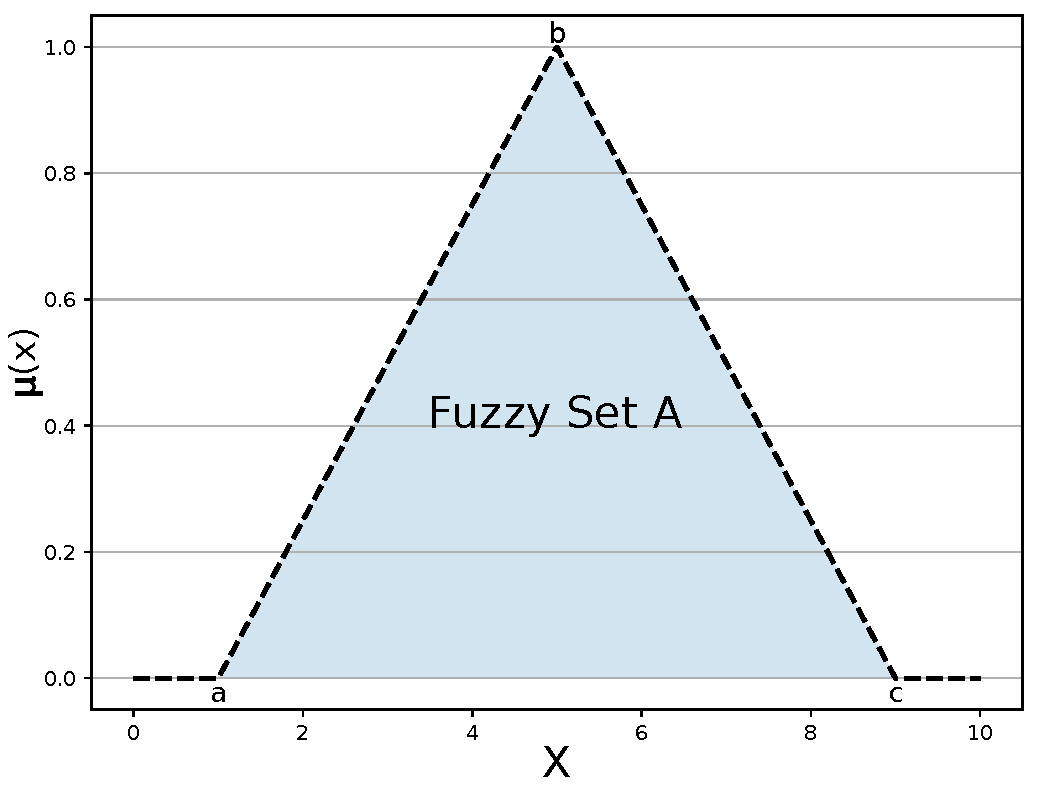
\includegraphics[width=2.9in]{images/triangular_fuzzy_number.pdf}
    \caption{Triangular Fuzzy Set – Illustrative example of the triangular membership function used to represent linguistic terms.
    }
    \label{fig_triangular_mf}
\end{figure}

Furthermore, given that a linguistic variable comprises several linguistic terms, it is also necessary to define a triangular fuzzy number $(a, b, c)$ for each of these terms. An example of a linguistic variable and it linguistic terms is presented in Table \ref{tab_fuzzy_numbers} and illustrated in Figure \ref{fig_linguistic_variables}. 

\begin{table}[!ht]
    \centering
    \caption{Example of Triangular Fuzzy Numbers for Linguistic Terms (Total Completion Time) – Values assigned to each fuzzy classification.}
    \label{tab_fuzzy_numbers}
    \begin{tabular}{lp{\twocolumns}}
        \toprule
        \textbf{Linguistic Term} & \textbf{Triangular Fuzzy Number (a, b, c)} \\
        \midrule
        very\_poor &  (12.50, 14.95, 14.95) \\
        poor & (10.05, 12.49, 14.94) \\
        medium\_poor & (7.58, 10.04, 12.49) \\
        fair & (5.13, 7.57, 10.02) \\
        medium\_good & (2.67, 5.12, 7.57) \\
        good & (0.22, 2.65, 5.10) \\
        very\_good &(0.20, 0.20, 2.65) \\
        \bottomrule
    \end{tabular}
\end{table}

The final concept required for the comprehension of our proposal is fuzzification. Fuzzification is a technique that provides a mechanism for transforming non-fuzzy values into linguistic terms. Hence, for a specific value $x \in X$, and a linguistic variable $L$ = $\{A_1, A_2, \cdots, A_n\}$, we determine the membership degree of $x$ with respect to every term within $L$. The linguistic term that has the highest membership degree is then selected as the most representative term for $x$. Formally:

\begin{equation}\label{eq_fuzzification}
    \delta_L(x) = \underset{l \in L}{\text{argmax}} \, \mu_l(x)~,
\end{equation}

This means that, using Equation \eqref{eq_fuzzification}, we can derive the corresponding triangular fuzzy number (TFN) associated with the most representative term for $x$.

To consolidate the knowledge of our proposed solution, an example is provided to illustrate how the fuzzification process is applied to determine the linguistic term associated with the total latency ($L^t_i$). For this purpose, we use the definitions outlined in Tables \ref{tab_fuzzy_numbers} and \ref{tab_ex_concepts}.

\begin{table}[!ht]
    \renewcommand{\arraystretch}{1.3}
    \setlength{\tabcolsep}{2.5pt}
    \caption{Fuzzy Logic Concepts Applied to Total Completion Time – Illustrative example of the fuzzification process and the selection of the most representative term.}\label{tab_ex_concepts}
    \centering
        \begin{tabular}{lp{\twocolumns}}
        \toprule
         \bfseries Concept & \bfseries Value \\
         \midrule
         Linguistic Variable & Total latency ($L^t_i$)\\
         Linguistic Terms &``$very\_poor$'', ``$poor$'', ``$medium\_poor$'', ``$fair$'', ``$medium\_good$'', ``$good$'', and ``$very\_good$'' \\
         Universe of Discourse & Set of possible values for total latency ($[0.2, 14.95]$ seconds) \\
        \botrule
        \end{tabular}
\end{table}

\begin{figure}[H]
    \centering
    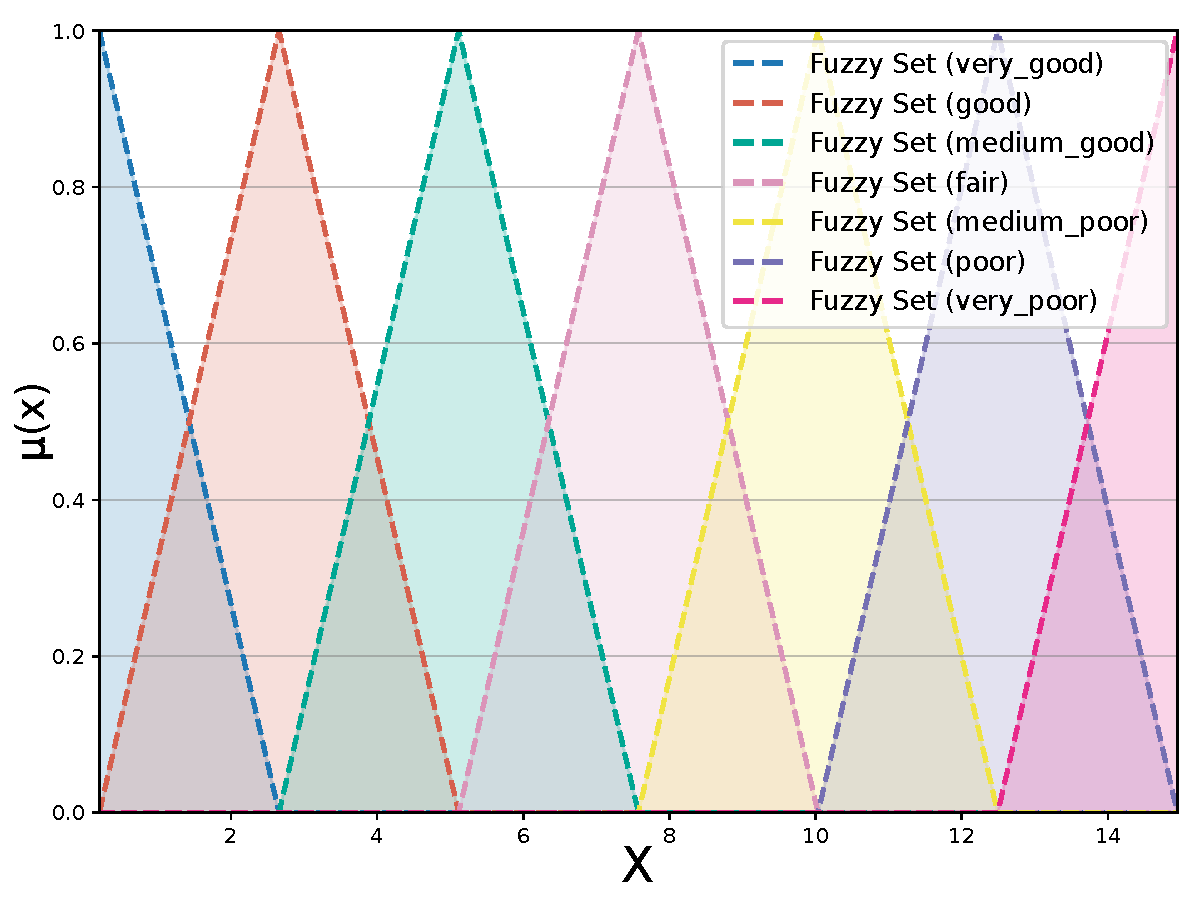
\includegraphics[width=2.9in]{images/latency.pdf}
    \caption{Linguistic Variable and Its Terms – Demonstrative example of the linguistic terms used to classify the total latency time.
    }
    \label{fig_linguistic_variables}
\end{figure}

Initially, we calculate the membership degree for an arbitrary $x=5.95$ using Equation \eqref{eq_triangular_mf} for each fuzzy set illustrated in Figure \ref{fig_linguistic_variables}. The results of these calculations are shown in Table \ref{tab_membership_degrees}. Finally, we complete the fuzzification process by applying Equation \eqref{eq_fuzzification}, which identifies the corresponding linguistic term as ``$medium\_good$'' due to its highest membership value of $0.66$. Based on this result, we obtain the corresponding triangular fuzzy number $(2.67, 5.12, 7.57)$.

\begin{table}[!ht]
    \centering
    \caption{Degrees of Membership for a Time of 5.95 Seconds – Association values for each linguistic term.}
    \label{tab_membership_degrees}
    \begin{tabular}{lc}
        \toprule
        \textbf{Linguistic Term} & \textbf{Membership Degree} \\
        \midrule
        very\_poor &  0.0 \\
        poor & 0.0 \\
        medium\_poor & 0.0 \\
        fair & 0.33 \\
        medium\_good & 0.66 \\
        good & 0.0 \\
        very\_good & 0.0 \\
        \bottomrule
    \end{tabular}
\end{table}

Finally, Tables \ref{tab_ex_concepts_energy} and \ref{tab_fuzzy_numbers_energy} illustrate how fuzzy logic was used to determine the linguistic term associated with the total energy consumption ($E^t_i$) and the corresponding TFN.


\begin{table}[!ht]
    \renewcommand{\arraystretch}{1.3}
    \setlength{\tabcolsep}{2.5pt}
    \caption{Fuzzy Logic Concepts Applied to Energy Consumption – Example of the fuzzification process to determine the term associated with energy consumption.
    }\label{tab_ex_concepts_energy}
    \centering
        \begin{tabular}{lp{\twocolumns}}
        \toprule
         \bfseries Concept & \bfseries Value \\
         \midrule
         Linguistic Variable & Total energy consumption ($E^t_i$)\\
         Linguistic Terms &``$very\_poor$'', ``$poor$'', ``$medium\_poor$'', ``$fair$'', ``$medium\_good$'', ``$good$'', and ``$very\_good$'' \\
         Universe of Discourse & Set of possible values for total energy consumption ($[5, 670]$ nJ/Cycle) \\
        \botrule
        \end{tabular}
\end{table}

\begin{table}[!ht]
    \centering
    \caption{Triangular Fuzzy Numbers for Linguistic Terms (Total Energy Consumption) – Representation of the fuzzy values assigned to each classification.
    }
    \label{tab_fuzzy_numbers_energy}
    \begin{tabular}{lp{\twocolumns}}
        \toprule
        \textbf{Linguistic Term} & \textbf{Triangular Fuzzy Number (a, b, c)} \\
        \midrule
        very\_poor &  (570.5, 620.3, 670.0) \\
        poor & (470.8, 520.6, 570.4) \\
        medium\_poor & (371.1, 420.9, 470.7) \\
        fair & (271.4, 321.2, 371.0) \\
        medium\_good & (171.7, 221.5, 271.3) \\
        good & (72.0, 121.8, 171.6) \\
        very\_good & (5.0, 38.5, 71.9) \\
        \botrule
    \end{tabular}
\end{table}

\section{Proposed Solution}\label{sec_fuzzy_topsis}
FOFF is an energy-efficient task offloading solution based on Fuzzy TOPSIS \cite{CHEN20001}, which is a multi-criteria decision-making (MCDM) method. 

In our work, we employ a modified version of this approach within the task offloading context, leveraging both its capacity to incorporate unlimited criteria when evaluating alternatives and its mathematical simplicity, which allows for rapid decision-making without introducing undue delays \cite{kahraman2008fuzzy}.

Algorithms \ref{alg_foff} and \ref{alg_fuzzy_topsis} demonstrate how we employ this technique to select the most suitable device for processing a task.

\begin{algorithm}
    \caption{Fuzzy Offloading (FOFF)}\label{alg_foff}
    \begin{algorithmic}[1]
        \Require Edge server list $M$, OBUI $U$, Task $T$, Linguistic variable for the total task latency $\zeta$, Linguistic variable for the total energy consumption $\varepsilon$, List of linguistic terms representing the weight of total task latency and total energy consumption $\omega$    \Ensure Selected device, Offloading ratio $\alpha$
    \State $array \gets fuzzy\_topsis(M, U, T, \zeta, \varepsilon, \omega)$
    \State \Return $array[0], 1$
    \end{algorithmic}
\end{algorithm}

Initially, as shown in Algorithm \ref{alg_foff}, it is necessary to specify the required input parameters for the task offloading decision-making process. These parameters are passed to the $fuzzy\_topsis$ function (line 1), which returns an ordered array of devices, ranked by suitability in descending order. Therefore, the device with the best combination of computational capacity ($f$), processing queue waiting time ($Q$), and energy consumption coefficient ($\kappa$) will be at the top of this array. Following this, FOFF selects the top-ranked device for task processing (line 2).

Algorithm \ref{alg_fuzzy_topsis} details the $fuzzy\_topsis$ function, regarding how it ranks the devices based on their characteristics to process a task. The description of our solution will proceed in two parts: first, we will explain the input parameters and their necessity; and second, we will describe the construction of the device ranking.

\begin{algorithm}
    \caption{Fuzzy TOPSIS function}\label{alg_fuzzy_topsis}
    \begin{algorithmic}[1]
    \Require Edge server list $\mathbf{M}$, OBUI $\mathbf{U}$, Task $\mathbf{T}$, Linguistic variable for total task latency $\zeta$, Linguistic variable for total energy consumption $\varepsilon$, List of linguistic terms representing the weight of total task latency and total energy consumption $\omega$
    \Ensure Selected device, Offloading ratio $\alpha$
    \Ensure Ranked devices by proximity index
    \State $\mathbf{\tilde{D}} \gets$ Create a decision matrix $\mathbf{\tilde{D}}_{m\times2}$ where $\mathbf{\tilde{D}}_{ij} = \left[ f(\delta_\zeta(L^t_i)), f(\delta_\varepsilon(E^t_i)) \right]$
    \State $\mathbf{\tilde{R}} \gets$ Create the normalized decision matrix $\mathbf{\tilde{R}}$ from $\mathbf{\tilde{D}}$ using Equation \eqref{eq_normalization_cost_chen}
    \State $\mathbf{\tilde{V}} \gets$ Multiply $\mathbf{\tilde{R}}$ by $\mathbf{\tilde{W}}$
    \State $\mathbf{A}^+ \gets$ Obtain the Positive Ideal Solution using the maximum values of $\mathbf{\tilde{V}}$
    \State $\mathbf{A}^- \gets$ Obtain the Negative Ideal Solution using the minimum values of $\mathbf{\tilde{V}}$
    \State $\mathbf{D}^+ \gets$ Calculate the distance of each alternative to $\mathbf{A}^+$
    \State $\mathbf{D}^- \gets$ Calculate the distance of each alternative to $\mathbf{A}^-$
    \State $\mathbf{C} \gets$ Calculate the proximity index of each alternative using $\mathbf{D}^+$ and $\mathbf{D}^-$
    \State $\textbf{ranking} \gets$ Order alternatives based on $\mathbf{C}$
    \State \Return $\textbf{ranking}$
    \end{algorithmic}
\end{algorithm}


\subsection{Input Parameters}

To understand Algorithm \ref{alg_fuzzy_topsis}, it is important to first define its input parameters as presented below:

\begin{enumerate}
    \item $M$: A list of characteristics for edge devices, including computational capacity ($f$), energy consumption coefficient ($\kappa$), and processing queue waiting time ($Q$).
    \item $OBUI$: The same characteristics ($f$, $\kappa$, and $Q$) but for the device installed in the vehicle.
    \item $T$: A variable representing the processing requirements of a given task.
    \item $\zeta$: A linguistic variable associated with the total task completion time.
    \item $\varepsilon$: A linguistic variable associated with the total energy consumption.
    \item $\omega$: A list of linguistic terms of importance associated with the total latency and total energy consumption for processing a task.
\end{enumerate}

The interval values for the linguistic terms of the linguistic variables $\zeta$ and $\varepsilon$ are defined dynamically as the simulation progresses. Specifically, when the OBUI receives information regarding the estimated task completion time, this value is segmented according to the seven linguistic terms established for $\zeta$. An identical approach is adopted to determine the energy consumption intervals for $\varepsilon$. Consequently, the interval definitions for $\zeta$ and $\varepsilon$ are continuously updated throughout the execution of the solution, accurately reflecting the current conditions of the system.

The initial step of Algorithm \ref{alg_fuzzy_topsis} (line 1) is the formation of the decision matrix. However, our construction of this matrix diverges from the traditional Fuzzy TOPSIS implementation. To appreciate this variation, it is essential to understand the original decision matrix construction methodology presented by Chen \textit{et al.} \cite{CHEN20001}.

In the context of a decision-making problem, multiple decision-makers, denoted as $DM_r$ ($r=1,\cdots,k$), may participate in the decision-making process. These decision-makers are responsible for evaluating the characteristics $Ch_j$ ($j=1,\cdots,m$) of each alternative $A_i$ ($i=1,\cdots,n$) using linguistic terms. For instance, a given decision-maker $DM_1$ may evaluate $Ch_1$ of alternative $A_1$ as ``\textit{very\_poor},'' while $DM_2$ may evaluate it as ``\textit{poor}.''

To address these uncertainties, Chen \textit{et al.} \cite{CHEN20001} proposed a method for aggregating these ratings using Equation \eqref{eq_integrate}, where $\tilde{x}_{ij}^K$ is the rating of the K-th decision-maker, and $\tilde{x}_{ij}$ is defined as a triangular fuzzy number.

\begin{equation}\label{eq_integrate}
    \tilde{x}_{ij} = \frac{1}{K} \left[ \tilde{x}_{ij}^1 + \tilde{x}_{ij}^2 + \dots + \tilde{x}_{ij}^k \right]
\end{equation}

To illustrate this, if two decision-makers rate two alternatives based on three of its characteristics, the resulting ratings would be organized as shown in Table \ref{tb_decision_makers}.

\newlength{\fivecolumns}
\setlength{\fivecolumns}{\dimexpr\columnwidth/5\relax} 

\begin{table}[!ht]
    \centering
    \caption{Example of Decision Makers' Evaluations – Comparison of alternatives based on three characteristics, with aggregated scores expressed as fuzzy numbers.
    }
    \label{tb_decision_makers}
    \begin{tabular}{llp{\fivecolumns}p{\fivecolumns}}
        \toprule
        \textbf{Alternative} & \textbf{Char.} & \textbf{$DM_1$ Rating} & \textbf{$DM_2$ Rating} \\
        \midrule
        \multirow{3}{*}{$A_1$}
        & $Ch_1$ &  $\tilde{x}_{11}^1$: very\_good & $\tilde{x}_{11}^2$: good \\
        & $Ch_2$ &  $\tilde{x}_{12}^1$: fair &  $\tilde{x}_{12}^2$: poor \\
        & $Ch_3$ & $\tilde{x}_{13}^1$: poor &  $\tilde{x}_{13}^2$: very\_poor \\
        \midrule
       \multirow{3}{*}{$A_2$}
        & $Ch_1$ &  $\tilde{x}_{21}^1$: good &  $\tilde{x}_{21}^2$: fair \\
        & $Ch_2$ & $\tilde{x}_{22}^1$: very\_poor &  $\tilde{x}_{22}^2$: medium\_poor \\
        & $Ch_3$ & $\tilde{x}_{23}^1$: fair & $\tilde{x}_{23}^2$: fair \\
        \bottomrule
    \end{tabular}
\end{table}

Therefore, to construct the decision matrix, Equation \eqref{eq_integrate} was used to aggregate the ratings resulting in $\mathbf{\tilde{D}_{2\times3}}$ (Matrix \eqref{eq_fuzzy_decision_matrix}).

\begin{equation}
    \label{eq_fuzzy_decision_matrix}
    \mathbf{\tilde{D}_{2\times3}} = 
    \begin{bmatrix}
        \tilde{x}_{11} & \tilde{x}_{12} & \tilde{x}_{13} \\
        \tilde{x}_{21} & \tilde{x}_{22} & \tilde{x}_{23}
    \end{bmatrix}
\end{equation}

Where each $\tilde{x}_{ij}$ represents a triangular fuzzy number resulting from the aggregation of decision-maker ratings for the $j$-th characteristic of the $i$-th alternative.

However, in the context of vehicular networks, it is impractical to have one or more human decision-makers constantly rating the characteristics of the edge servers and the OBUI. Therefore, it was necessary to specify an alternative method to replace the integration of ratings. 

To this end, we fuzzify each value for estimated total latency to complete a task ($L^t_i$), and the estimated total energy consumption ($E^t_i$) associated with each edge server and OBUI. For each of these values, it was necessary to create corresponding linguistic variables, which are passed as arguments to Algoritms \ref{alg_foff} and \ref{alg_fuzzy_topsis} using the symbols $\zeta$, and $\varepsilon$, respectively.

Therefore, the decision matrix is constructed using these notation:

\begin{equation}
    \label{eq_proposed_decision_matrix}
    \mathbf{\tilde{D}_{m\times2}} = 
    \begin{bmatrix}
    \delta_\zeta(L^t_1) & \delta_\varepsilon(E^t_1) \\
    \delta_\zeta(L^t_2) & \delta_\varepsilon(E^t_2) \\
    \vdots & \vdots \\
    \delta_\zeta(L^t_m) & \delta_\varepsilon(E^t_m)
    \end{bmatrix}
\end{equation}

where $m$ is the number of processing devices.

However, it is essential to clearly define how to associate linguistic terms (e.g., $\delta_\zeta(L^t_1)$ or $\delta_\varepsilon(E^t_1)$) with triangular fuzzy numbers to enable Fuzzy TOPSIS to effectively rank the best alternatives. This association is formalized as follows:

\begin{equation}
    \label{eq_lt_to_tfn}
    \delta_L(x) \xrightarrow{f} \text{TFN} = (a, b, c),
\end{equation}

where $f$ represents a function that formalizes the association rule between linguistic terms and fuzzy numbers. Various approaches can be employed to define $f$, including tabular methods, parametric functions, or heuristic algorithms \cite{kahraman2008fuzzy}.

In this way, the method by which we are creating the decision matrix in our proposal is presented in Matrix \eqref{eq_proposed_decision_matrix_final}.

\begin{equation}
    \label{eq_proposed_decision_matrix_final}
    \mathbf{\tilde{D}_{m\times2}} = 
    \begin{bmatrix}
    f(\delta_\zeta(L^t_1)) & f(\delta_\varepsilon(E^t_1)) \\
    f(\delta_\zeta(L^t_2)) & f(\delta_\varepsilon(E^t_2)) \\
    \vdots & \vdots  \\
    f(\delta_\zeta(L^t_m)) & f(\delta_\varepsilon(E^t_m))
    \end{bmatrix}
\end{equation}

\subsection{Construction of the Device Ranking}
In this subsection, we will detail each step of Algorithm \ref{alg_fuzzy_topsis} that contributes to the construction of the device ranking. 

The decision matrix ($\mathbf{\tilde{D}}$) requires normalization to enable a fair comparison across all device characteristics. Therefore, before presenting the normalization procedure, we must first define the concepts of benefit and cost criteria.

Benefit criteria are parameters for which higher values contribute more significantly to the pursuit of an optimal solution. The objective is to maximize these criteria when selecting an alternative.

Conversely, cost criteria are parameters for which lower values are more desirable, and thus must be minimized when choosing appropriate alternatives. In this work, task completion time and energy consumption are defined as cost criteria.

As specified by \cite{CHEN20001}, we derive the normalized matrix $\mathbf{\tilde{R}}$ from $\mathbf{\tilde{D}}$ using the following equation for each criterion, according Equation \eqref{eq_normalization_cost_chen}. This derivation is presented in line 2 of Algorithm \ref{alg_fuzzy_topsis}.


\begin{equation}
    \label{eq_normalized_matrix_chen}
    \mathbf{\tilde{R}} = [\tilde{r}_{ij}]_{m \times n}
\end{equation}

\begin{equation}
    \label{eq_normalization_cost_chen}
    \begin{split}
    \tilde{r}_{ij} = \left(\frac{l_j^-}{c_{ij}}, \frac{l_j^-}{b_{ij}}, \frac{l_j^-}{a_{ij}}\right), \\
    \text{where } l_j^- = \min_{i=1 \ldots m} a_{ij} \text{ (for cost criteria)}
\end{split}
\end{equation}

Having completed the normalization step, it is necessary to establish the relative importance of each criterion in the ranking process. For this purpose, a linguistic variable with predefined values is created to represent these relative importance levels, as detailed in Table \ref{tab_fuzzy_importance} and illustrated in Figure \ref{fig_importance_weight}.

\begin{table}[!ht]
    \centering
    \caption{Triangular Fuzzy Numbers for Criteria Weighting – Fuzzy values associated with the importance levels of each criterion.}
    \label{tab_fuzzy_importance}
    \begin{tabular}{lp{\twocolumns}}
        \toprule
        \textbf{Linguistic Term} & \textbf{Triangular Fuzzy Number (a, b, c)} \\
        \midrule
        very\_low (vl) & (0.0, 0.0, 0.17) \\
        low (l) & (0.0, 0.17, 0.33) \\
        medium\_low (ml) & (0.17, 0.33, 0.50) \\
        medium (m) & (0.33, 0.50, 0.67) \\
        medium\_high (mh) & (0.50, 0.67, 0.83) \\
        high (h) & (0.67, 0.83, 1.00) \\
        very\_high (vh) & (0.83, 1.00, 1.00) \\
        \bottomrule
    \end{tabular}
\end{table}

\begin{figure}[H]
    \centering
    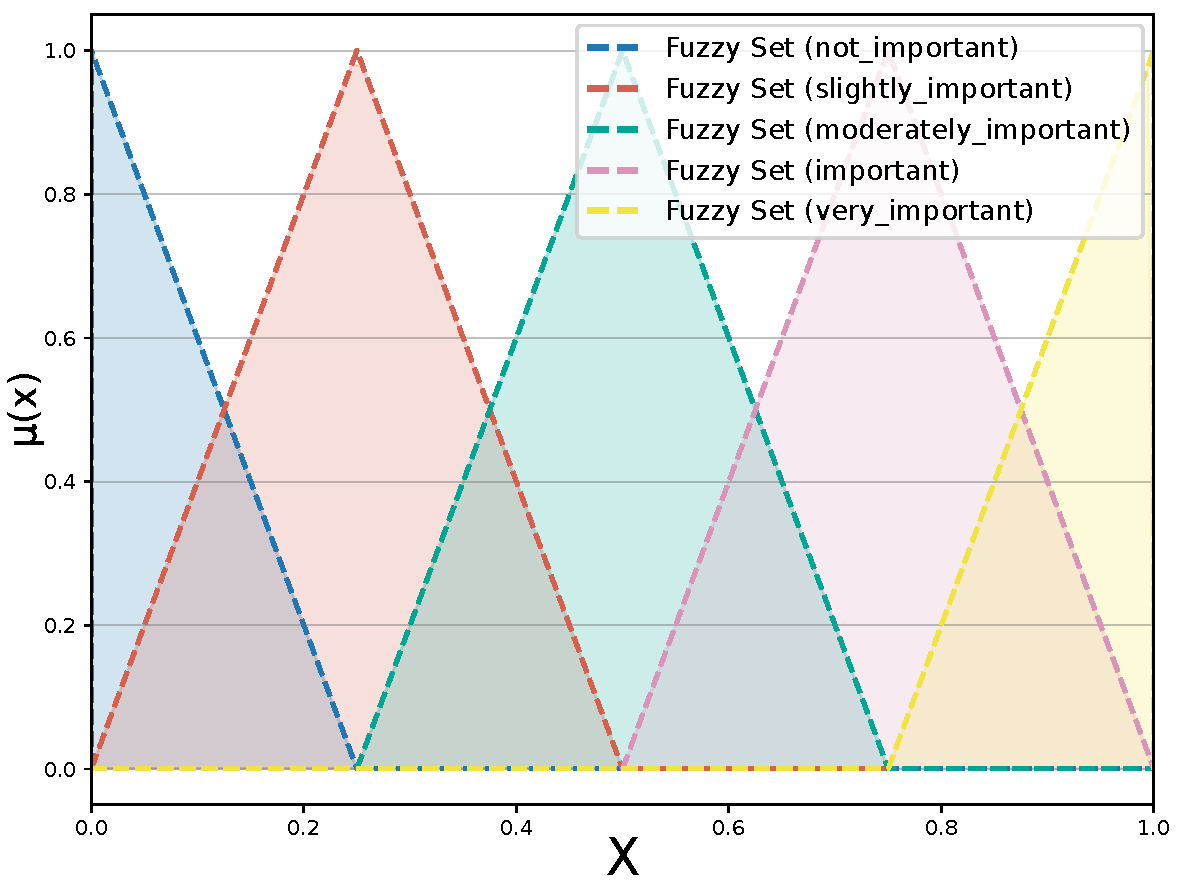
\includegraphics[width=2.9in]{images/importance_weight.pdf}
    \caption{Linguistic Variables for Criteria Weighting – Representation of the fuzzy values assigned to the importance of each criterion in the decision-making process.}
    \label{fig_importance_weight}
\end{figure}

To integrate these importance levels into the overall process (Algorithm \ref{alg_fuzzy_topsis}, line 3), we have to use the weight vector to define each metric's significance as described by Equation \eqref{eq:v_tilde}.

\begin{equation}\label{eq:v_tilde}
    \begin{split}
    \mathbf{\tilde{V}} = [\tilde{v}_{ij}]_{m \times n} \\
    \mathbf{\tilde{V}} = \mathbf{\tilde{D}} \otimes \mathbf{\tilde{W}}
    \end{split}
\end{equation}

The symbol $\otimes$ indicates the element-wise multiplication operation wich involves multiplying triangular fuzzy numbers on a one-to-one basis for each pair of corresponding elements.

In Fuzzy TOPSIS, the Positive Ideal Solution (PIS, $A^+$) and the Negative Ideal Solution (NIS, $A^-$) are fundamental concepts for ranking alternatives. The PIS and NIS represent, respectively, the best and worst possible values for each criterion. By using these reference points, each alternative is evaluated against the PIS and NIS, thereby facilitating comparisons among all alternatives.

Considering $A^+$, let $\tilde{v}_{ij} = (a_{ij}, b_{ij}, c_{ij})$ be a triangular fuzzy number with $\tilde{v}_{ij} \in \mathbf{\tilde{V}}$. For a benefit criterion ($j \in B$), the positive ideal vector is defined as $\tilde{v}^+_j = (a^+_{j}, b^+_{j}, c^+_{j})$, where:

\begin{equation}
    \begin{split}
    a^+_{j} = \max_{i=1,\dots,m} a_{ij}, \\
    b^+_{j} = \max_{i=1,\dots,m} b_{ij}, \\
    c^+_{j} = \max_{i=1,\dots,m} c_{ij}.
    \end{split}
\end{equation}

For a cost criterion ($j \in C$), the positive ideal vector is calculated using:

\begin{equation}
    \begin{split}
    a^+_{j} = \min_{i=1,\dots,m} a_{ij}, \\
    b^+_{j} = \min_{i=1,\dots,m} b_{ij}, \\
    c^+_{j} = \min_{i=1,\dots,m} c_{ij}.
    \end{split}
\end{equation}

For instance, consider two triangular fuzzy numbers defined as $\tilde{v}_{1j} = (2, 6, 6)$ and $\tilde{v}_{2j} = (3, 5, 7)$. The positive ideal vector for a benefit criterion $(j \in B)$, which maximizes each component, will be:

\begin{equation}
\tilde{v}^+_j = (3, 6, 7).
\end{equation}

Conversely, for a cost criterion $(j \in C)$, which minimizes each component, the positive ideal vector will be:

\begin{equation}
\tilde{v}^+_j = (2, 5, 6).
\end{equation}

Therefore, the PIS is specified using Equation \eqref{eq_positive_ideal_solution}:

\begin{equation}\label{eq_positive_ideal_solution}
    \mathbf{A^+} = \{ \tilde{v}^+_1, \cdots, \tilde{v}^+_n \}.
\end{equation}

Mathematically, the NIS is represented as shown in Equation \eqref{eq_negative_ideal_solution}:

\begin{equation}\label{eq_negative_ideal_solution}
    \mathbf{A^-} = \{ \tilde{v}^-_1, \cdots, \tilde{v}^-_n \}.
\end{equation}

Here, $A^-$ is a set of negative ideal values $\tilde{v}^-_j$ for all criteria $j$, where $j = 1, \cdots, n$ and $\tilde{v}^-_j = (a^-_{j}, b^-_{j}, c^-_{j})$. These values are derived differently depending on whether the criterion is a benefit or a cost.

For a benefit, the NIS is calculated by minimizing each component of the triangular fuzzy numbers across all alternatives:

\begin{equation}
    \begin{split}
    a^-_{j} = \min_{i=1,\dots,m} a_{ij}, \\
    b^-_{j} = \min_{i=1,\dots,m} b_{ij}, \\
    c^-_{j} = \min_{i=1,\dots,m} c_{ij}.
    \end{split}
\end{equation}

Conversely, for a cost criterion the NIS is calculated by maximizing each component of the triangular fuzzy numbers:

\begin{equation}
    \begin{split}
    a^-_{j} = \max_{i=1,\dots,m} a_{ij}, \\
    b^-_{j} = \max_{i=1,\dots,m} b_{ij}, \\
    c^-_{j} = \max_{i=1,\dots,m} c_{ij}.
    \end{split}
\end{equation}

In this way, it is possible to compute the relative closeness of each alternative to both $A^+$ (line 4 of Algorithm \ref{alg_fuzzy_topsis}) and $A^-$ (line 5 of Algorithm \ref{alg_fuzzy_topsis}) by using Euclidean distances, as described in Equations \ref{eq_d_plus} (line 6 of Algorithm \ref{alg_fuzzy_topsis}) and \ref{eq_d_minus} (line 7 of Algorithm \ref{alg_fuzzy_topsis}), respectively. 

\begin{equation}\label{eq_d_plus}
    D_i^+ 
    = \sqrt{
        \sum_{j=1}^n 
        \left[
            d(\tilde{v}_{ij}, \tilde{v}_j^+)
        \right]^2
    }, 
    \quad \text{for } i=1,\dots,m,
\end{equation}

\begin{equation}\label{eq_d_minus}
    D_i^- 
    = \sqrt{
        \sum_{j=1}^n 
        \left[
            d(\tilde{v}_{ij}, \tilde{v}_j^-)
        \right]^2
    }, 
    \quad \text{for } i=1,\dots,m,
\end{equation}

where $d(\tilde{v}_{ij}, \tilde{v}_j^+)$ and $d(\tilde{v}_{ij}, \tilde{v}_j^-)$ represent the calculation of the difference between each vertex of two TFNs.

Figure \ref{fig_relative_closeness} illustrates how an alternative is positioned relative to both ideal solutions. These calculations make it possible to identify which alternatives are closer to the PIS and farther from the NIS.

\begin{figure}[H]
    \centering
    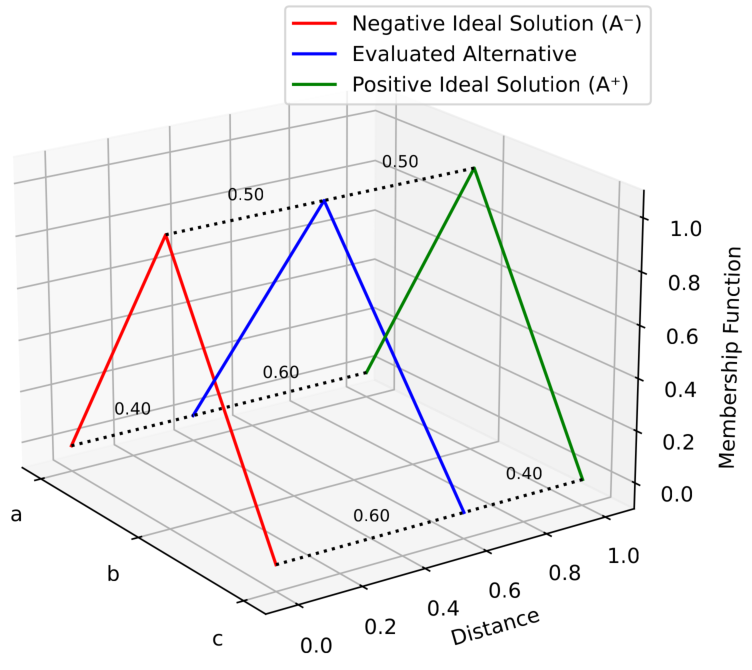
\includegraphics[width=2.7in]{images/relative_closeness_of_the_alternative_to_ideal_solutions.pdf}
    \caption{Relative Closeness of Alternatives to Ideal Solutions – Visualization of the distances of the alternatives from the ideal points (positive and negative).
}
    \label{fig_relative_closeness}
\end{figure}

Based on the calculated distances, the relative proximity (Equation \eqref{eq_relative_proximity}, line 8 of Algorithm \ref{alg_fuzzy_topsis}) of each alternative to the ideal solutions is determined. 

\begin{equation}\label{eq_relative_proximity}
C_i = \frac{D_i^-}{D_i^+ + D_i^-}
\end{equation}

This proximity value is then used to rank the alternatives, and the device (OBUI or Edge Server) that achieves the highest proximity is selected for task processing.

Finally, the ranking is sorted in descending order in line 9, and returned in line 10 of Algorithm \ref{alg_fuzzy_topsis}.

\subsection{Framework Architecture}

In our proposed solution, each OBUI is capable of making its own offloading decisions without relying on a central controller. As a result, the system exhibits high scalability, as each embedded device autonomously manages its own task offloading processes. Jiang et al. \cite{jiang2019toward}, in their review, highlight that the ability of each device to evaluate edge server characteristics — such as processing capacity, latency, and energy consumption — enables autonomous selection of the most appropriate resource for executing each task. This decentralized approach eliminates the need for a central controller and significantly enhances system scalability.

Moreover, the framework architecture used in our experiments was based on the architecture proposed in \cite{de2021context}, excluding vehicle-to-vehicle communication via WAVE (Wireless Access in Vehicular Environments).

\section{Experiments, Sensitivity Analysis and Results}\label{sec_experiments}

In this Section, we present the experiments, the sensitivity analysis and the results obtained from applying the proposed solution. We compare the FOFF against other offloading strategies (ROFF \cite{de2021context}, GTT \cite{de2021context}, FP-Sched \cite{10757894}, and HOFF \cite{sadatdiynov2023intelligent}) in two distinct scenarios: 1) \textit{Challenging} and 2) \textit{Balanced}. 

A \textit{Challenging Scenario} is defined by an OBUI with low computational capacity and high energy consumption, along with edge servers that possess high computational capacity but also a high energy consumption coefficient (Table \ref{tab_scenario_01}). In contrast, a \textit{Balanced Scenario} consists exclusively of devices with moderate energy consumption and adequate computational capacity (Table \ref{tab_scenario_02}).


\begin{table}[ht!]
    \centering
    \caption{Devices and Parameters in the \textit{Challenging Scenario} – Specifications of the devices employed in the simulation of a challenging environment.}
    \label{tab_scenario_01}
    \begin{tabular}{lcc}
    \toprule
    \textbf{Device} & \textbf{CPU (GHz)} & \textbf{nJ/Cycle} \\
    \midrule
    Edge 00 & 2 &  90\\
    Edge 01 & 4 & \textbf{670}\\
    Edge 02 & 2 & 5\\
    Edge 03 & 4 & \textbf{345}\\
    Edge 04 & 2 & 88\\
    OBUI    & 1 & \textbf{1310}\\
    \botrule
    \end{tabular}
\end{table}

\begin{table}[ht!]
    \centering
    \caption{Devices and Parameters in the \textit{BalancedScenario} – Specifications of the devices used in the simulation of a balanced environment.}
    \label{tab_scenario_02}
    \begin{tabular}{lcc}
    \toprule
    \textbf{Device} & \textbf{CPU (GHz)} & \textbf{nJ/Cycle} \\
    \midrule
    Edge 00 & 2 &  5\\
    Edge 01 & 3 & 11\\
    Edge 02 & 2 & 10\\
    Edge 03 & 4 & 23\\
    Edge 04 & 2 & 12\\
    OBUI    & 1 & 20\\
    \botrule
    \end{tabular}
\end{table}

The simulations were performed on a computer with 40 GB RAM and a 13th Gen Intel(R) Core(TM) i5-13450HX 2.40 GHz processor. These simulations were based on the scenario illustrated in Figure \ref{fig_scenario}, where the vehicle's OBUI can connect to five edge servers, each with distinct characteristics.

\begin{figure}[H]
    \centering
    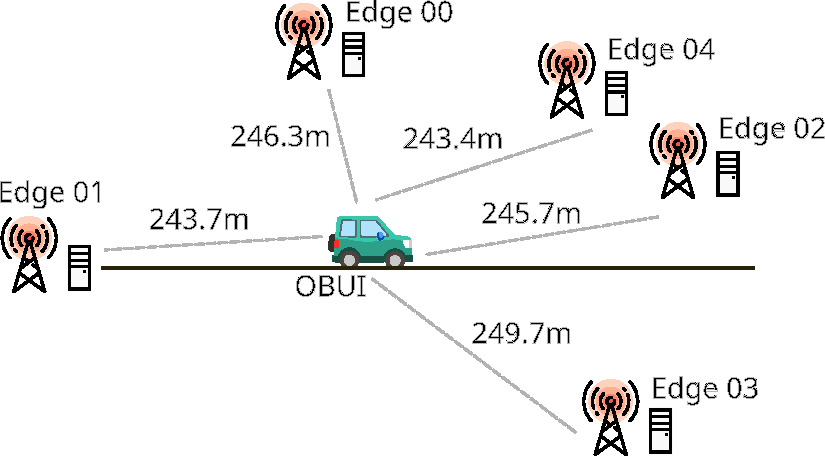
\includegraphics[width=2.9in]{images/scenario.pdf}
    \caption{Vehicular Scenario with VEC and 5G Communication --- Overview of the simulation environment adopted in this study.
    }\label{fig_scenario}
\end{figure}

These scenarios were chosen to assess how well FOFF adapts to different conditions. In each simulation run, we generated 1,000 tasks and created a 100 distinct scenarios, yielding a total of 100,000 offloading decisions.

We modeled tasks with varying input data sizes, and CPU cycle requirements for processing. Thus, in our simulations, a vehicle may generate lightweight tasks (with a few million cycles and low latency priority) or heavy, encompassing diverse load heterogeneity scenarios. This variability was incorporated precisely to evaluate the performance of the FOFF scheme under realistic conditions where tasks are not identical.

It was necessary to compare our approach with other offloading techniques. For this, we adapted some of the solutions developed in \cite{de2021context} to our simulation environment. The goal is to evaluate how solutions based on a random strategy and adapted version of greedy strategies (\textit{Greedy Task by Task} - GTT \cite{de2021context}, \textit{Fully Partitioned Scheduling} - FP-Sched \cite{10757894}, and \textit{Hybrid Offloading} - HOFF \cite{sadatdiynov2023intelligent}) perform in deliberately challenging and balanced environments and, based on this baseline, assess how a fuzzy approach addresses such a challenge.

The \textit{Random Offloading} - ROFF \cite{de2021context} solution generates a random value using a uniform distribution to decide whether a task will be processed locally or offloaded to an edge server. The FP-Sched \cite{10757894} strategy is based on a fully partitioned scheduling mechanism, in which each task must be executed entirely on a single edge device. Devices are evaluated within discrete time slots, and candidate devices are selected based on their ability to complete the task considering transmission time, execution time, and availability during the current slot. The strategy applies a First-Fit Decreasing Utilization (FFDU) policy to assign tasks to the earliest available suitable device, avoiding overload. The GTT estimates the total time required to send, process, and receive a task for each available edge device. Therefore, the selected server is the one that offers high CPU capacity, minimal queue time, and proximity to the client. 

The HOFF is a NSGA-II --- based method tackles the offloading decision as a constrained multi-objective optimization problem. It generates a population of candidate offloading configurations --- each representing a set of binary decisions for processing tasks either locally or at the edge --- and evaluates them with respect to both energy consumption and latency. By employing non-dominated sorting and crowding distance mechanisms, the algorithm iteratively refines the candidate solutions, effectively balancing trade-offs between processing delays, energy usage, and available computational capacity. Ultimately, the optimal offloading decision is selected from the Pareto-optimal set, ensuring that tasks are assigned to the edge server that not only meets the system constraints but also minimizes overall execution time and energy expenditure.

The simulation parameters for both scenarios are presented in Table \ref{tab_simulation_parameters}.

\begin{table}[ht!]
    \centering
    \caption{Main Simulation Parameters --- Configurations adopted for the experiments.}
    \label{tab_simulation_parameters}
    \begin{tabular}{p{\twocolumns}l}
    \toprule
    \textbf{Parameter} & \textbf{Value} \\
    \midrule
    \textbf{General} \\
    Simulation time & 1500 seconds \\
    \# of tasks & 1000 per simulation \\
    \# of simulations & 100x per scenario \\ 
    Available edge servers & All \\ 
    CPU capacity of devices in both scenarios & [1, 4] GHz \\
    Energy consumption of devices in \textit{Challenging Scenario} & [5, 1310] nJ/Cycle \\
    Energy consumption of devices in \textit{BalancedScenario} & [5, 23] nJ/Cycle \\
    \\
    \textbf{5G} \\
    Communication range & 250 meters \\ 
    Radio propagation model & Free-Space \\
    Data rate & 450 Mbps \\
    \botrule
    \end{tabular}
\end{table}

\subsection{Sensitivity Analysis}\label{sec_sensitive_analysis}

This section presents a comprehensive sensitivity analysis of the FOFF with respect to the importance weights assigned to the energy consumption and latency criteria. The analysis examines how different linguistic weight combinations affect the FOFF's performance in terms of energy efficiency and task completion time.

\subsubsection{Analysis Setup}

The sensitivity analysis was conducted using a \textit{Challenging Scenario} involving heterogeneous devices with diverse computational capabilities. We tested 13 different weight configurations, where each weight combination is represented by linguistic terms: very low (vl), low (l), medium low (ml), medium (m), medium high (mh), high (h), and very high (vh). The first weight ($\omega_1$) corresponds to latency importance, while the second weight ($\omega_2$) corresponds to energy consumption importance.

For each configuration, we measured performance improvements compared to GTT and ROFF baseline strategies in terms of: Percentage of energy efficiency improvements, percentage of task completion time improvement, and average of energy and latency improvements.

\subsubsection{Effect of Weight Selection on Energy Efficiency}

\begin{figure}[H]
    \centering
    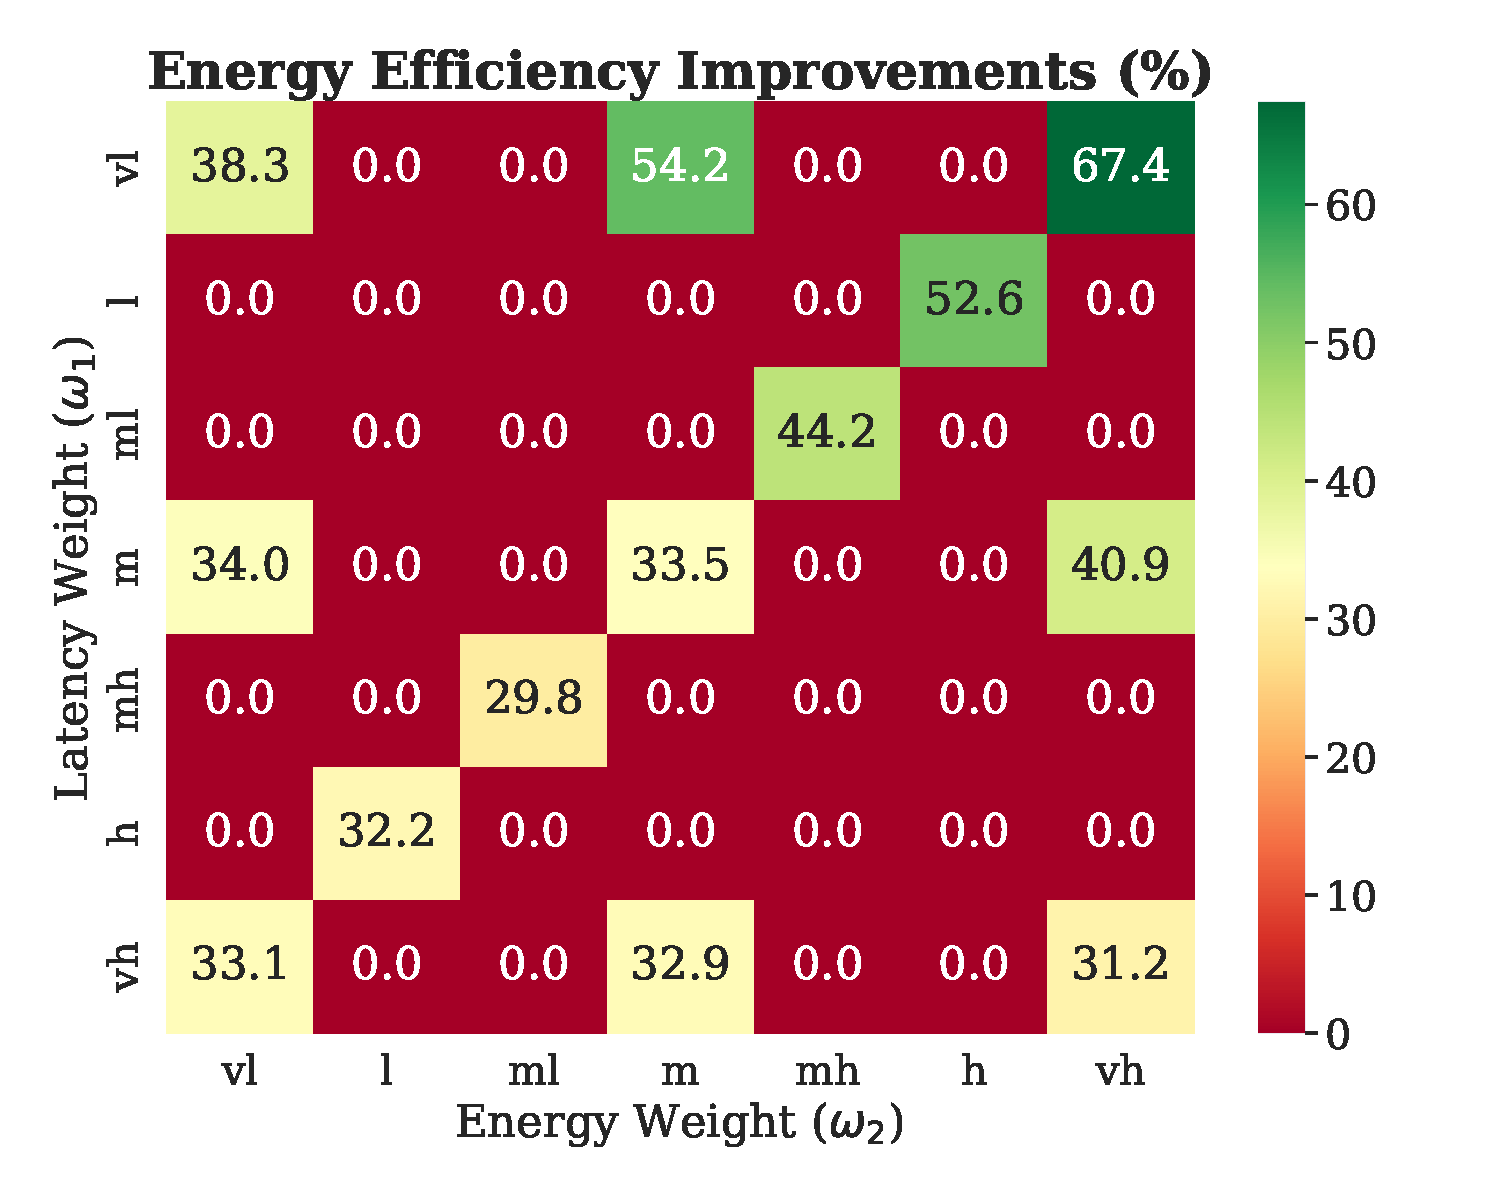
\includegraphics[width=2.9in]{images/energy_heatmap_FOFF.pdf}
    \caption{A Heatmap of FOFF energy efficiency improvements for distinct weight settings relative to the GTT and ROFF baseline solutions in challeging scenario.}\label{fig_energy_heatmap}
\end{figure}

Figure \ref{fig_energy_heatmap} illustrates the sensitivity of energy efficiency to different weight configurations. The analysis reveals that energy efficiency is highly responsive to weight selection, with improvements ranging from 29.8\% to 67.4\%.

The highest energy efficiency improvement (67.4\%) was achieved with the $\omega$=[vl,vh] configuration, which assigns very low importance to latency and very high importance to energy. Other notable configurations include $\omega$=[vl,m] with 54.2\% improvement and $\omega$=[l,h] with 52.6\% improvement.

The results demonstrate that prioritizing energy considerations through higher $\omega_2$ values consistently leads to better energy efficiency outcomes. However, this effect is particularly pronounced when combined with lower $\omega_1$ values, indicating that energy-latency trade-offs must be carefully considered.

\subsubsection{Effect of Weight Selection on Task Completion Time Performance}

\begin{figure}[H]
    \centering
    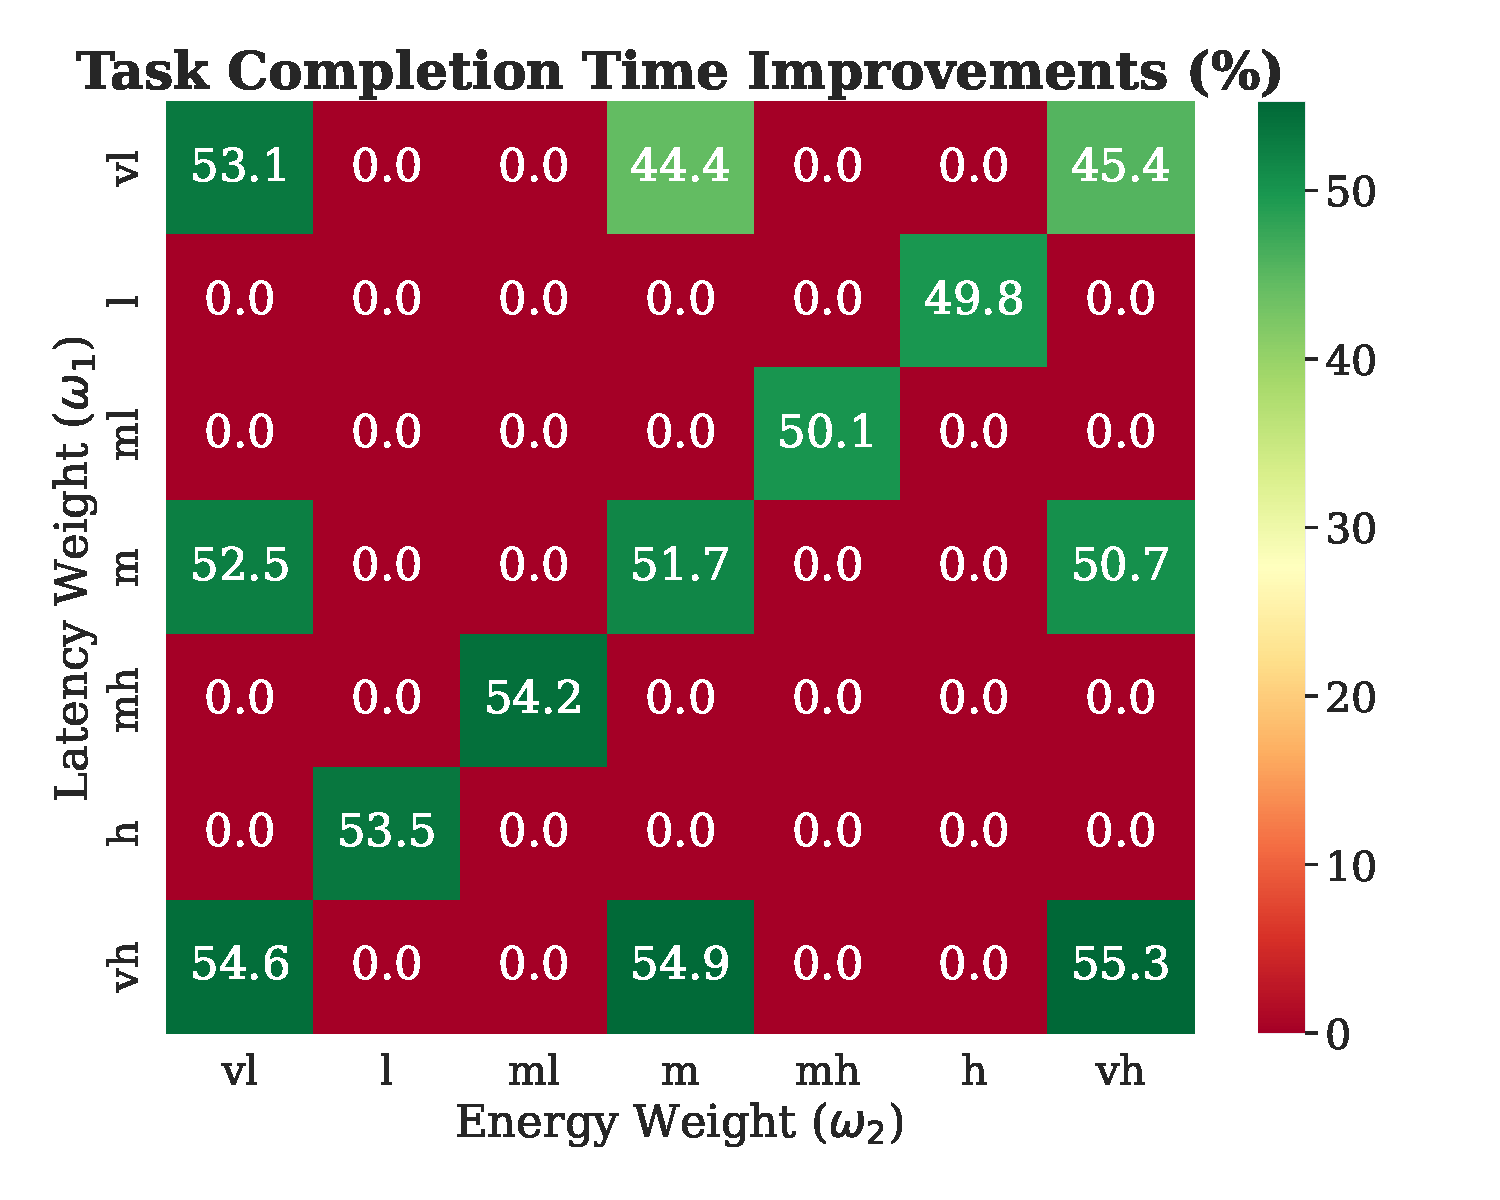
\includegraphics[width=2.9in]{images/latency_heatmap_FOFF.pdf}
    \caption{A Heatmap of FOFF task completion time improvements for distinct weight settings relative to the GTT and ROFF baseline solutions in challeging scenario.}\label{fig_latency_heatmap}
\end{figure}

As shown in Figure \ref{fig_latency_heatmap}, latency performance also exhibits significant sensitivity to weight selection, with improvements ranging from 44.4\% to 55.3\%. 

Interestingly, several configurations achieved latency improvements exceeding 50\%, with the highest improvement (55.3\%) observed in the $\omega$=[vh,vh] configuration. Other effective configurations include $\omega$=[vh,m] (54.9\%), $\omega$=[mh,ml] (54.2\%), and $\omega$=[vh,vl] (54.6\%).

The results indicate that latency performance benefits from higher $\omega_1$ values, as expected, but it remains relatively robust across various weight combinations. This suggests that FOFF can maintain good latency performance even when energy considerations are prioritized.

\subsubsection{Energy-Task Completion Time Trade-off Analysis}
\newlength{\fourcolumns}
\setlength{\fourcolumns}{\dimexpr\columnwidth/5\relax} 

\begin{table}[ht!]
    \centering
    \caption{Energy and Task Completion Time Improvements for Different FOFF Weight Configurations Relative to baseline GTT in Challeging Scenario.}
    \label{tab_energy_latency_tradeoff}
    \begin{tabular}{cp{\fourcolumns}p{\fourcolumns}p{\fourcolumns}}
    \toprule
    \textbf{$\omega$} & \textbf{Energy Improvements (\%)} & \textbf{Task Completion Time Improvements (\%)} & \textbf{Average Improvements (\%)} \\
    \midrule
    (vl, vh) & 67.44 & 45.43 & 56.44 \\
    (vl, m) & 54.19 & 44.43 & 49.31 \\
    (l, h) & 52.55 & 49.81 & 51.18 \\
    (ml, mh) & 44.19 & 50.06 & 47.13 \\
    (m, vh) & 40.87 & 50.70 & 45.78 \\
    (vl, vl) & 38.27 & 53.11 & 45.69 \\
    (m, vl) & 33.99 & 52.51 & 43.25 \\
    (m, m) & 33.55 & 51.68 & 42.62 \\
    (vh, vl) & 33.07 & 54.56 & 43.81 \\
    (vh, m) & 32.87 & 54.87 & 43.87 \\
    (h, l) & 32.15 & 53.53 & 42.84 \\
    (vh, vh) & 31.17 & 55.26 & 43.21 \\
    (mh, ml) & 29.84 & 54.22 & 42.03 \\
    \botrule
    \end{tabular}
    \end{table}

Table \ref{tab_energy_latency_tradeoff} presents the energy-latency trade-off for different FOFF weight configurations. The analysis reveals a clear but non-linear relationship between energy efficiency and latency improvements. The $\omega$=[l,h] configuration stands out with 52.6\% energy improvement and 49.8\% latency improvement, offering a balanced performance profile. Other balanced configurations include $\omega$=[ml,mh] (44.2\% energy, 50.1\% latency) and $\omega$=[m,vl] (34.0\% energy, 52.5\% latency).

For applications with specific priorities, specialized configurations can be selected: Energy-critical applications: $\omega$=[vl,vh] (67.4\% energy, 45.4\% latency) and Latency-critical applications: $\omega$=[vh,vh] (31.2\% energy, 55.3\% latency)

\subsubsection{Implications and Recommendations}

The sensitivity analysis yields several important insights for FOFF implementation:

\begin{enumerate}
    \item Weight selection significantly impacts performance, with potential improvements varying by more than 35\% for energy efficiency and 10\% for latency.
    \item For general-purpose applications requiring balanced performance, the $\omega$=[l,h] configuration offers the best compromise between energy efficiency and latency.
    \item In energy-constrained environments (e.g., battery-powered devices), the $\omega$=[vl,vh] configuration provides maximum energy savings while maintaining acceptable latency.
    \item For delay-sensitive applications (e.g., real-time processing), the $\omega$=[vh,vh] configuration ensures minimum latency while still providing substantial energy savings compared to baseline approaches.
    \item The robust latency performance across various configurations suggests that FOFF can maintain good responsiveness even when optimizing for energy efficiency.
\end{enumerate}

This sensitivity analysis demonstrates that FOFF provides a flexible and effective mechanism for adapting the offloading strategy to different operational requirements and constraints. System administrators can select appropriate weight configurations based on their specific performance priorities without requiring modifications to the underlying algorithm.

\subsection{Total Energy Consumption Results}
As observed in Figure \ref{fig_energy_results} (\textit{Challenging} Scenario), FOFF demonstrated an average energy consumption of 5.07 J $\pm$ 1.67. Compared to GTT, which recorded an energy consumption of 12.06 J $\pm$ 2.98, FOFF achieved a reduction of 57.96\%, highlighting its energy efficiency. In the case of ROFF, which reached 126088.60 J $\pm$ 2731.28, FOFF achieved a 99.99\% reduction. HOFF recorded 3067.46 J $\pm$ 597.43. This indicates that FOFF achieved an approximately 99.83\% reduction in energy consumption compared to HOFF. Compared to FP-Sched, which recorded an energy consumption of 277.40 J $\pm$ 158.46, FOFF achieved a reduction of 98.17\%.

\begin{figure}[H]
    \centering
    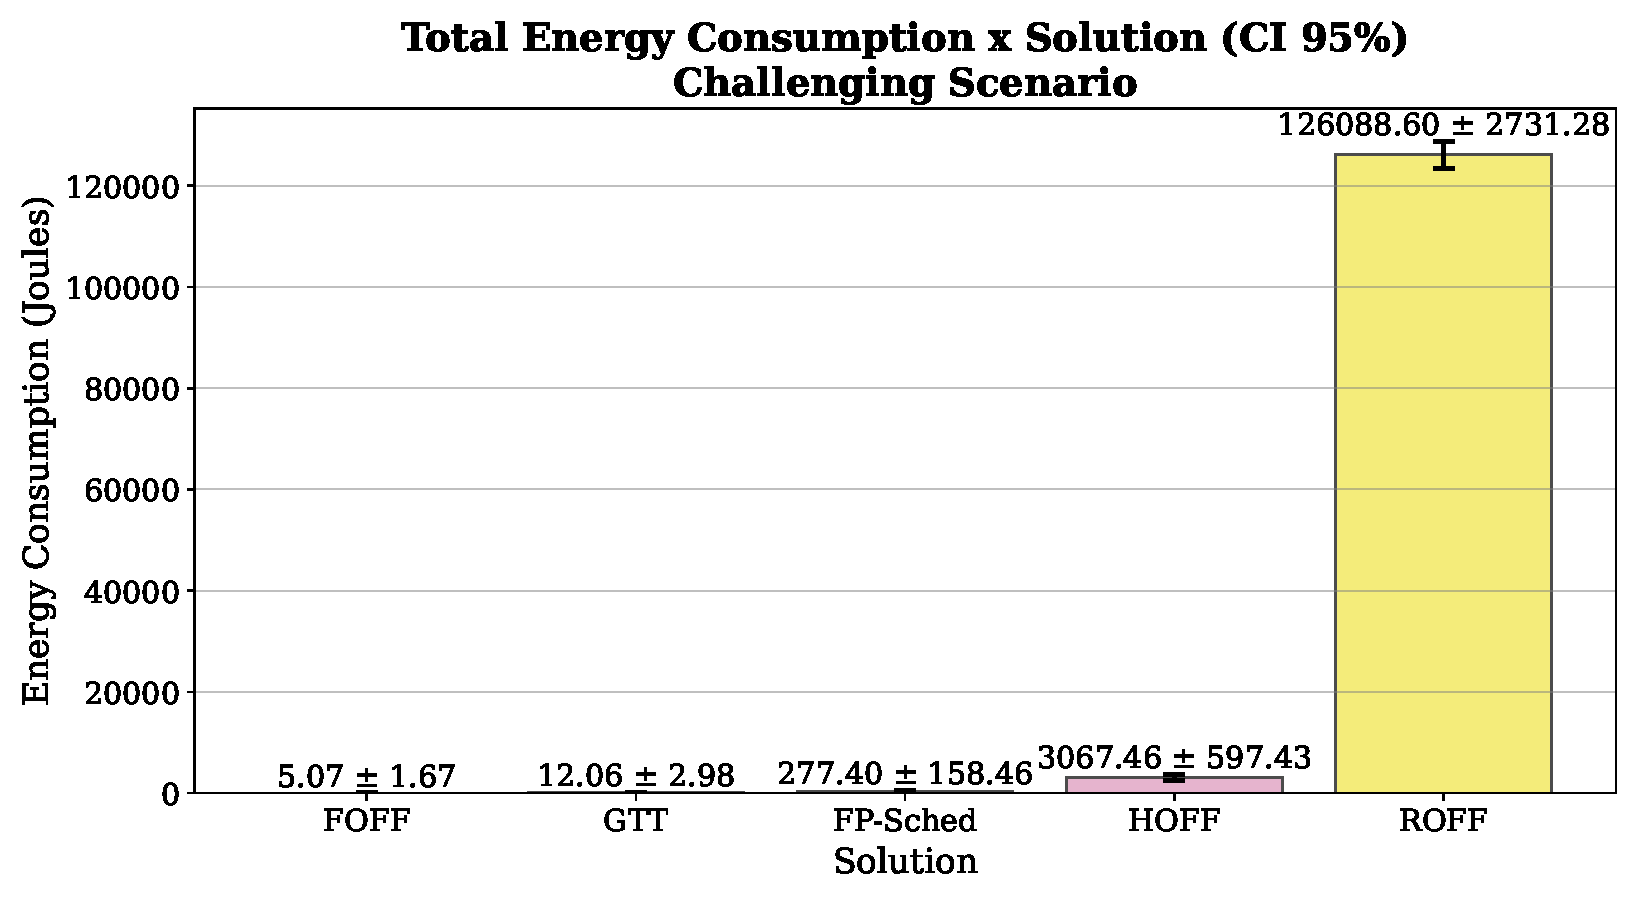
\includegraphics[width=2.9in]{images/challenging_energy_cost.pdf}
    \caption{Comparison of Total Energy Consumption in the \textit{Challenging Scenario} – Analysis of the average energy consumption obtained for task processing.}
    \label{fig_energy_results}
\end{figure}

The results obtained using a \textit{BalancedScenario} are shown in Figure \ref{fig_energy_results_balanced}, where FOFF demonstrated an average energy consumption of 3.06 J $\pm$ 1.35. Compared to ROFF, which recorded an energy consumption of 125916.24 J $\pm$ 2753.51, FOFF achieved a reduction of 99.99\%, showcasing its energy efficiency. In the case of GTT, which had an energy consumption of 10.97 J $\pm$ 3.00, FOFF achieved a reduction of 72.11\%. Furthermore, when comparing FOFF with HOFF, which presented an energy consumption of 3078.57 J $\pm$ 599.09, FOFF demonstrated a significant reduction of 99.90\%. Lastly, compared to FP-Sched, which recorded an energy consumption of 272.74 J $\pm$ 159.76, FOFF achieved a reduction of 98.88\%.

\begin{figure}[H]
    \centering
    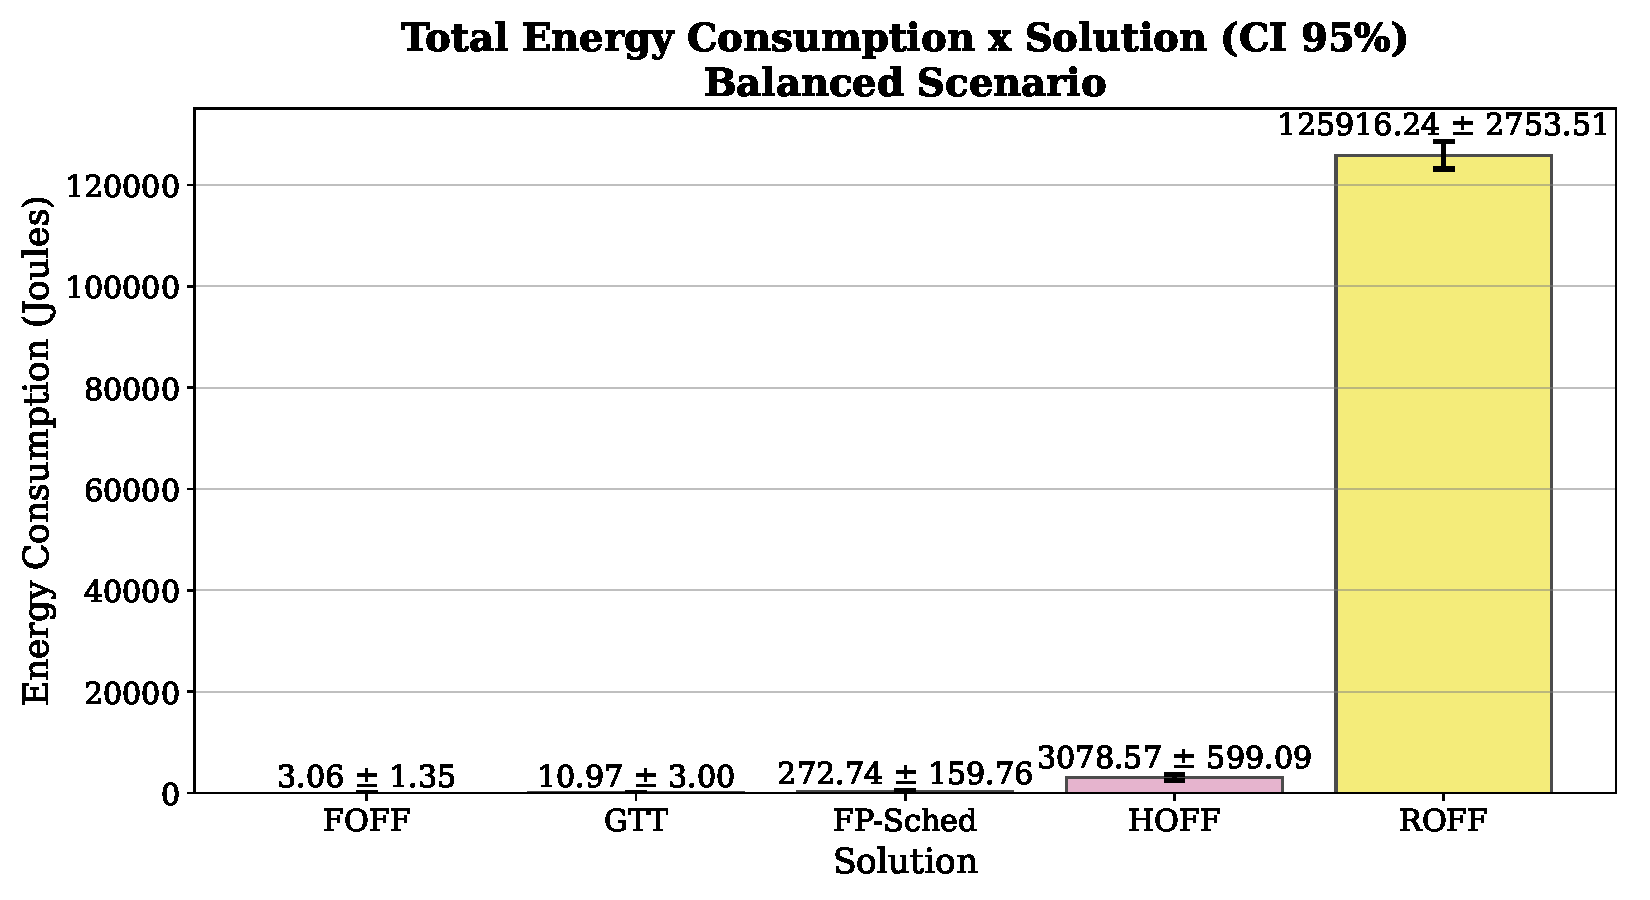
\includegraphics[width=2.9 in]{images/balanced_energy_cost.pdf}
    \caption{Comparison of Total Energy Consumption in the \textit{BalancedScenario} – Evaluation of the average energy consumption for task processing.}
    \label{fig_energy_results_balanced}
\end{figure}

\subsection{Task Completion Time Results}
In the \textit{Challenging Scenario}, the FOFF algorithm achieved a total task completion time of 21.24 s $\pm$ 1.48, as illustrated in Figure \ref{fig_latency_results_challenging}. Compared to GTT (21.28 s $\pm$ 1.46), FOFF achieved a reduction of about 0.19\%. ROFF, employing a random strategy, reached a total task completion time of 16468.66 s $\pm$ 360.63, indicating a reduction of 99.87\% by FOFF. When compared to HOFF (413.81 s $\pm$ 75.47), FOFF demonstrated a significant reduction of 94.87\%. Additionally, FP-Sched recorded 56.49 s $\pm$ 21.09, with FOFF achieving a 62.40\% reduction. On a per-task basis, FOFF averaged approximately 0.212 s, while GTT averaged 0.213 s, FP-Sched 0.565 s, HOFF 4.138 s, and ROFF 164.687 s.

\begin{figure}[H]
    \centering
    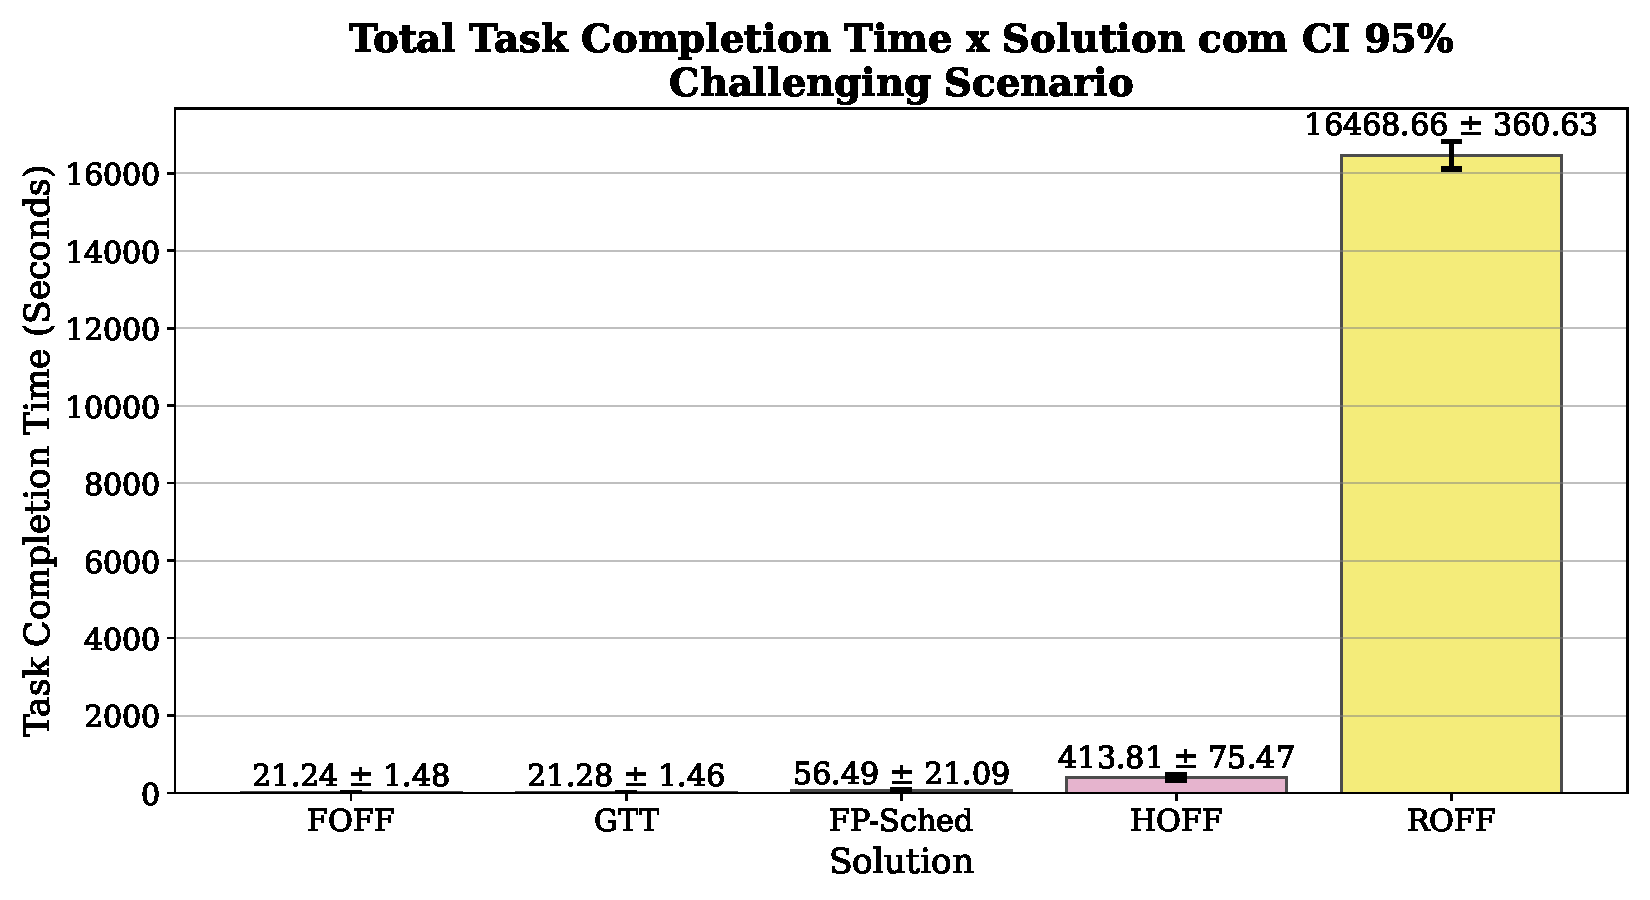
\includegraphics[width=2.9 in]{images/challenging_processed_time.pdf}
    \caption{Comparison of Overall Processing Time in the Challenging Scenario – Analysis of end-to-end latency for task execution.}
    \label{fig_latency_results_challenging}
\end{figure}

In the \textit{BalancedScenario}, the FOFF algorithm demonstrated strong performance, achieving a total task completion time of 21.20 s $\pm$ 1.48, as illustrated in Figure \ref{fig_latency_results_balanced}. When compared to GTT (21.33 s $\pm$ 1.45), FOFF attained a reduction of approximately 0.61\%. In relation to ROFF (16452.18 s $\pm$ 358.52), it achieved a substantial reduction of 99.87\%. When compared to HOFF (419.01 s $\pm$ 76.45), FOFF demonstrated a significant reduction of 94.94\%. Compared to FP-Sched (56.26 s $\pm$ 20.97), FOFF achieved a reduction of 62.32\%. These findings confirm that FOFF's strategy, which also considers energy consumption, effectively minimizes latency. Examining the per-task completion time shows that FOFF and GTT required about 0.212 s and 0.213 s, respectively. In contrast, FP-Sched took 0.563 s, HOFF took 4.190 s, and ROFF took 164.522 s per task.

\begin{figure}[H]
    \centering
    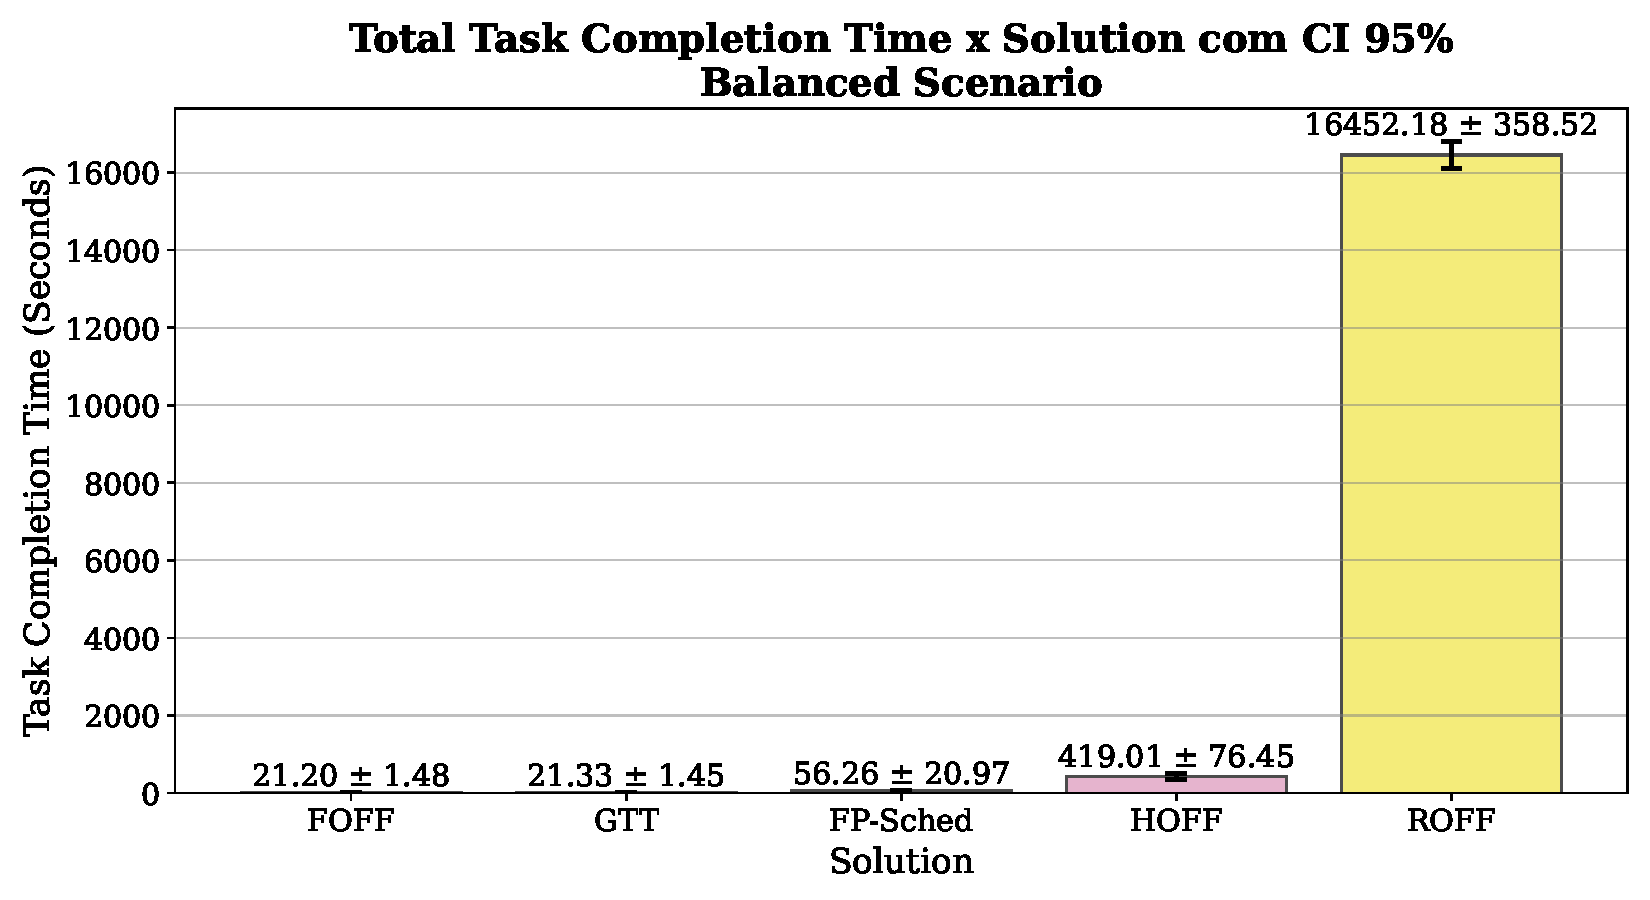
\includegraphics[width=2.9in]{images/balanced_processed_time.pdf}
    \caption{Comparison of Total Processing Time in the \textit{BalancedScenario} – Analysis of the total observed latency in task processing.}
    \label{fig_latency_results_balanced}
\end{figure}

\subsection{Discussion}
As demonstrated in our experiments, the proposed approach exhibits adaptability in both scenarios. In the experiment involving high-computational-capacity devices with high energy costs (\textit{Challenging Scenario}), FOFF reduced energy consumption in 57.96\% while achieving 0.19\% lower total latency compared to GTT.

In the \textit{BalancedScenario}, FOFF adapted autonomously without requiring weight adjustments, yielding a 0.61\% improvement in latency over GTT and 99.90\% reduction in energy consumption compared to HOFF. This adaptability underscores FOFF's capability to operate across diverse environments without the need for manual tuning. When compared to HOFF, FOFF achieved impressive reductions in task completion time --- 94.87\% in the Challenging Scenario and 94.94\% in the \textit{BalancedScenario} --- while maintaining significantly lower energy consumption. These findings suggest that FOFF and GTT solutions are particularly well-suited for vehicular applications with stringent latency requirements, with FOFF offering the additional benefit of energy efficiency.

Despite not employing a greedy technique, FOFF outperformed GTT in both scenarios. These results demonstrate the effectiveness of the proposed fuzzy logic-based solution in making intelligent offloading decisions that balance the competing demands of processing speed and energy conservation.

\begin{table}[ht]
    \centering
    \caption{Wilcoxon signed-rank test between FOFF and baseline methods in challenge scenario with $\omega$=[vl,vh]}
    \label{tab:wilcoxon}
    \begin{tabular}{lllll}
    \toprule
    \textbf{Scenario} & \textbf{Metric} & \textbf{Method} & \textbf{p-value}\\
    \midrule
    Balanced   & Energy & GTT       & 0.0000 \\
    Balanced   & Energy & FP-Sched  & 0.6229 \\
    Balanced   & Energy & HOFF      & 0.0000 \\
    Balanced   & Energy & ROFF      & 0.0000 \\
    Balanced   & Time   & GTT       & 0.2807 \\
    Balanced   & Time   & FP-Sched  & 0.0072 \\
    Balanced   & Time   & HOFF      & 0.0000 \\
    Balanced   & Time   & ROFF      & 0.0000 \\
    \midrule
    Challenging & Energy & GTT       & 0.0032 \\
    Challenging & Energy & FP-Sched  & 0.3586 \\
    Challenging & Energy & HOFF      & 0.0000 \\
    Challenging & Energy & ROFF      & 0.0000 \\
    Challenging & Time   & GTT       & 0.7117 \\
    Challenging & Time   & FP-Sched  & 0.0053 \\
    Challenging & Time   & HOFF      & 0.0000 \\
    Challenging & Time   & ROFF      & 0.0000 \\
    \bottomrule
    \end{tabular}
\end{table}
    
In the \textit{BalancedScenario}, FOFF’s mean energy usage was substantially lower than that of GTT, HOFF, and ROFF, with Wilcoxon signed-rank tests confirming that these reductions are statistically significant (each comparison yielded $p < 0.01$). FOFF also achieved lower average energy consumption than FP-Sched; however, this particular difference was not statistically significant at the 5\% level, indicating comparable energy efficiency between FOFF and FP-Sched in this case. In terms of task completion time, FOFF completed tasks faster than FP-Sched, HOFF, and ROFF by a wide margin. These pairwise improvements in completion time were all statistically significant as well (Wilcoxon $p < 0.01$ for each). Against GTT, FOFF attained essentially the same task completion time. The slight gap observed was not significant ($p > 0.05$), indicating that FOFF matches GTT’s performance. Notably, FOFF manages to equal the fastest baseline (GTT) in completion time while using far less energy. Overall, under balanced conditions FOFF either significantly outperforms or at least matches the best baseline on both metrics, highlighting its robust advantages in efficiency and task completion time.

In the more demanding \textit{Challenging Scenario}, FOFF maintained its performance edge, underscoring the robustness of its approach under heavier workloads. FOFF continued to consume significantly less energy than GTT, HOFF, and ROFF (Wilcoxon tests, $p < 0.01$ in all comparisons), closely mirroring the improvements seen in the balanced case. When compared to FP-Sched, FOFF again exhibited a much lower mean energy consumption; due to the high variability in FP-Sched’s outcomes, however, this difference did not reach statistical significance ($p > 0.05$). This suggests that even in a challenging environment, FOFF is at least as energy-efficient as FP-Sched, and markedly more efficient than the other baselines.

FOFF also continued to deliver faster task completion times than nearly all baselines in the \textit{Challenging Scenario}. It finished tasks significantly sooner than FP-Sched, HOFF, and ROFF (all $p < 0.01$ in the Wilcoxon signed-rank tests), despite the increased difficulty of this scenario. As in the balanced condition, FOFF’s completion time was on par with GTT (no statistically significant difference, $p > 0.05$), meaning FOFF again matches the fastest baseline’s performance. The consistency of these results across both scenarios attests to FOFF’s robustness: the algorithm sustains its low energy consumption and swift task completion even under challenging conditions, significantly outperforming the baseline approaches in most comparisons.

\section{Conclusion}\label{sec_conclusion}
This paper proposed an innovative energy-efficient task offloading solution for 5G-VEC-enabled vehicular networks. By integrating fuzzy TOPSIS and multi-criteria decision-making, our approach effectively addressed critical challenges arising from dynamic vehicular environments, optimizing task allocation to significantly minimize energy consumption.

The experimental results validate the effectiveness of the proposed solution in reducing energy consumption under challenging conditions. Notably, Fuzzy Offloading successfully processed all assigned tasks, achieving notable energy savings and lower processing times compared to traditional greedy offloading methods. Specifically, FOFF reduced energy consumption by approximately $57.96\%$ and improved processing latency by around $0.19\%$ in \textit{Challenging Scenario}, underscoring its capability to manage conflicting objectives.

Future work will focus on extending the proposed solution to incorporate additional contextual parameters, such as vehicle speed and real-time network fluctuations. Furthermore, we will investigate the performance of our approach in large-scale mobility scenarios. There is significant potential for integrating advanced machine learning techniques, particularly deep reinforcement learning—to enable dynamic adaptation to rapidly changing environmental conditions. Finally, expanding the evaluation framework to larger and more diverse vehicular scenarios will ensure comprehensive validation and reinforce the applicability of the proposed solution across various use cases and network configurations.


%%===========================================================================================%%
%% If you are submitting to one of the Nature Portfolio journals, using the eJP submission   %%
%% system, please include the references within the manuscript file itself. You may do this  %%
%% by copying the reference list from your .bbl file, paste it into the main manuscript .tex %%
%% file, and delete the associated \verb+\bibliography+ commands.                            %%
%%===========================================================================================%%

\bibliographystyle{sn-mathphys-num}
\bibliography{sn-article}% common bib file
%% if required, the content of .bbl file can be included here once bbl is generated
%%\input sn-article.bbl


\end{document}
